\documentclass{beamer}
\usetheme{JuanLesPins}
\usepackage{epsfig, graphics, graphicx,subfigure, amsmath}
\usepackage[spanish]{babel}

[mathscr]{eucal}
%\psdraft
\title{cap\'itulo teor\'ia funcional de la densidad}
\begin{document}
	\frame{\titlepage}
	\section{contenidos}
	\frame{\frametitle{contenidos} \tableofcontents}
	\section{teor\'ia de Hartree-Fock}
	\frame{\frametitle{Perspectiva DFT}
		\begin{figure}[!hbt]
			\centering
			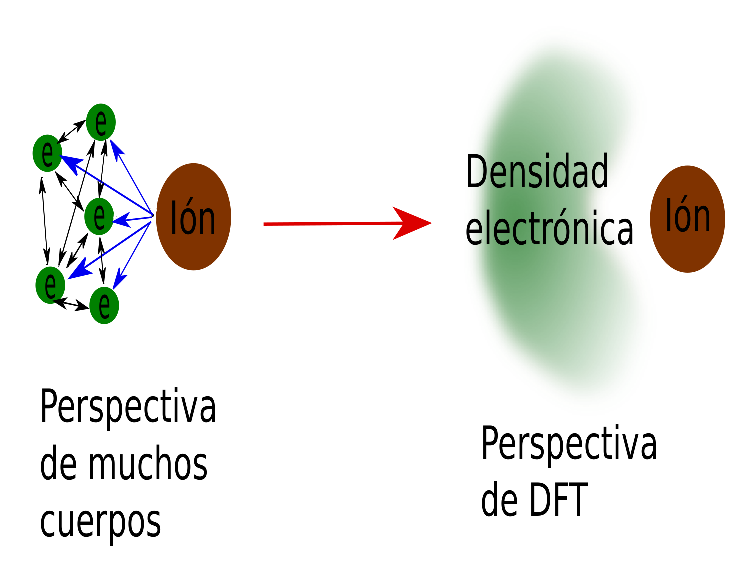
\epsfig{file=figuras/perspectivaDFT.eps, width=6.0cm,height=6.0cm}
			\caption{idea de la teor\'ia funcional de la densidad que consiste en sustituir las interacciones de muchos cuerpos con una interacci\'on promedio por medio de la densidad electr\'onica.}
			\label{im:dftIdea}
		\end{figure}
	}
	\frame{\frametitle{ec. de Schr\"odinger}
		\begin{itemize}
			\item El hamiltoniano  de muchos cuerpos es:
			\begin{multline}
			\hat H = - \frac{\hbar ^2}{2 m_e} \sum_{i} \nabla_{i}^2 - \sum_{i,I} \frac{Z_I e^2}{\vert \pmb{r_i} - \pmb{R_I} \vert}+ \frac{1}{2} \sum_{i \not= j}  \frac{e^2}{|\pmb{r_i} - \pmb{r_j} |}\\
			- \sum_{I} \frac{\hbar^2}{2 M_I} \nabla_I^2 + \frac{1}{2} \sum_{I \not= J} \frac{Z_I Z_J e^2}{|\pmb{R_I}-\pmb{R_J}|}  \label{ec:sh} 
			\end{multline}
			\pause
			\item Se puede utilizar la aproximac\'on de Born-Oppenheimer con el siguiente hamiltoniano
			\begin{equation}
			\hat H = \hat T + \hat V_{ext} + \hat V_{int}+E_{II} \label{ec:shelectron}
			\end{equation}
		\end{itemize}
	
	}
    \frame{
    	\begin{equation}
    	\hat{T} = \sum_{i} -\frac{1}{2} \nabla_{i}^2 \label{ec:shT}
    	\end{equation}
    	\pause
    	\begin{equation}
    	\hat{V}_{ext} = \sum_{i,I} V_I (|\pmb{r_i}-\pmb{R_I}|) \label{ec:shVex}
    	\end{equation}
    	\pause
    	\begin{equation}
    	\hat{V}_{int} = \frac{1}{2} \sum_{i \not= j} \frac{1}{|\pmb{r_i}-\pmb{r_j}|} \label{ec:shVint}
    	\end{equation}
    	
    }
    \frame{\frametitle{Ecuaci\'on de un solo cuerpo }
    	\begin{itemize}
    		\item Se trata de llegar a una ecuaci\'on de un solo cuerpo:
    		\begin{equation}
    		\hat H _{eff} \Psi_{i,s} (\pmb{r}) = \left [ -\frac{\hbar^2}{2m_e} \nabla^2 + V_{eff}^{s} \right]\Psi_{i,s} (\pmb{r}) = \varepsilon_i ^{s} \Psi_{i,s} (\pmb{r})  \label{ec:shuncuerpo}
    		\end{equation}
    		\pause
    		
    		\item La funci\'on de onda se puede escribir como un determinante de Slater:
    		\begin{equation}
    		\Psi = \frac{1}{\sqrt{N !}}
    		\begin{vmatrix}
    		\phi_1 (\pmb{r}_1, s_1) & \phi_1 (\pmb{r}_2, s_2) & \phi_1 (\pmb{r}_3, s_3) & \cdots & \phi_1 (\pmb{r}_N, s_N) \\
    		\phi_2 (\pmb{r}_1, s_1) & \phi_2 (\pmb{r}_2, s_2) & \phi_2 (\pmb{r}_3, s_3) & \cdots & \phi_2 (\pmb{r}_N, s_N)\\
    		\phi_3 (\pmb{r}_1, s_1) & \phi_3 (\pmb{r}_2, s_2) & \phi_3 (\pmb{r}_3, s_3) & \cdots & \phi_3 (\pmb{r}_N, s_N) \\
    		&  \vdots                     & \vdots                      &  \ddots & \vdots\\
    		\phi_N (\pmb{r}_1, s_1) & \phi_N (\pmb{r}_2, s_2) & \phi_N (\pmb{r}_3, s_3) & \cdots & \phi_N (\pmb{r}_N, s_N) \\
    		
    		\end{vmatrix} \label{ec:slater}
    		\end{equation}
    		
    	\end{itemize}
    }
    \frame{\frametitle{Algunos valores de expectaci\'on \'utiles}
    	\begin{itemize}
    		\item Energ\'ia:
    		\begin{equation}
    		E= \langle \Psi | \hat{H} | \Psi \rangle \label{ec:energia}
    		\end{equation}
    		\pause
    		\item densidad de electrones:
    		\begin{equation}
    		n_{s ', s} (\pmb{r ', r} ) = \delta_{s',s} \sum_{i} \psi_{i,s} ^{ *} (\pmb{r'}) n_{i,s} \psi_{i,s } (\pmb{r})  \label{ec:densidadr}
    		\end{equation}
    		\pause
    		\item magnetizaci\'on:
    		\begin{equation}
    		\pmb{m} (\pmb{r}) = - \mu_{B} \sum_{s,s '} \pmb{\sigma}_{s,s'} n_{s ', s }(\pmb{r}) \label{ec:magn}
    		\end{equation}
    		
    		
    	\end{itemize}
    }
    \frame{ \frametitle{Algunos valores de expectaci\'on \'utiles} 
    	con componentes:
    	\begin{subequations} \label{ec:compm}
    		\begin{gather}
    		m_x (\pmb{r})= -2 \mu_{B} Re~ n_{\uparrow, \downarrow} (\pmb{r}) \label{ec:compm1}\\
    		m_y (\pmb{r})= -2 \mu_{B} Im~ n_{\uparrow, \downarrow} (\pmb{r}) \label{ec:compm2}\\
    		m_z (\pmb{r}) = - \mu_{B} [n_{\uparrow, \uparrow} (\pmb{r})- n_{\downarrow, \downarrow} (\pmb{r})] \label{ec:compm3}
    		\end{gather}
    	\end{subequations}
    }
    \frame{\frametitle{C\'alculo de la enrg\'ia}
    	Suponendo que no se cuento con acople spin-\'orbita se puede dividir $ \phi_i (\pmb{r}_i, s_i)$ en una parte dependiente de la posici\'on $ \psi_{i,s} (\pmb{r_j}) $ y otra que dependa del spin $s$, $ \alpha_i (s_j)$ y el c\'alculo de la energ\'ia es
    	\begin{multline}
    	E =\sum_{i,s} \int d\pmb{r} \psi_{i,s}^* (\pmb{r})\left [ -~\frac{1}{2} \nabla^2 + V_{ext} (\pmb{r}) \right] \psi_{i,s} (\pmb{r}) +E_{II}\\
    	+\frac{1}{2} \sum_{i,j,s_i,s_j} \int d\pmb{r} d\pmb{r'} \psi_{i,s_i}^* (\pmb{r}) \psi_{j,s_j}^* (\pmb{r '}) \frac{1}{|\pmb{r}-\pmb{r'}|} \psi_{i,s_i} (\pmb{r}) \psi_{j,s_j} (\pmb{r '})\\
    	-\frac{1}{2} \sum_{i,j,s} \int d\pmb{r} d\pmb{r'} \psi_{i,s}^* (\pmb{r}) \psi_{j,s}^* (\pmb{r '}) \frac{1}{|\pmb{r}-\pmb{r'}|} \psi_{j,s} (\pmb{r}) \psi_{i,s} (\pmb{r '}) \label{ec:ecEnergia}
    	\end{multline}
    }
    \frame{\frametitle{Minimizaci\'on de la energ\'ia}
    	El siguiente paso es minimizar la energ\'ia del sistema (ec. \ref{ec:ecEnergia}) utilizando los multiplicadores de Lagrange y usando como restricci\'on que las funciones de onda son ortonormales y se obtienen las ecuaciones de Hartree-Fock:
    	\begin{multline}
    	\left[ -~\frac{1}{2} \nabla^2+ V_{ext} (\pmb{r})+ \sum_{j,s_j} \int d \pmb{r'} \psi_{j,s_j}^* (\pmb{r'}) \psi_{j,s_j} (\pmb{r'}) \frac{1}{|\pmb{r} - \pmb{r'}|}  \right] \psi_{i,s} (\pmb{r}) \\
    	- \sum_{j} \int d \pmb{r'} \psi_{j,s}^* (\pmb{r'}) \psi_{i,s} (\pmb{r'}) \frac{1}{|\pmb{r} - \pmb{r'}|} \psi_{j,s} (\pmb{r}) = \varepsilon_{i,s} \psi_{i,s} (\pmb{r}) \label{ec:hartree_fock}
    	\end{multline} 
    }
   \frame{\frametitle{Potencial de intercambio y correlaci\'on}
   	se define la densidad de dos part\'iculas:
   	\begin{multline}
   	n(\pmb{r},s; \pmb{r'},s' )= \left\langle \sum_{I \not= J} \delta (\pmb{r}- \pmb{r_i}) \delta (s-s_i) (\pmb{r'}- \pmb{r_j}) \delta (s'-s_i) )  \right\rangle \\
   	= N(N-1) \sum_{s_3,s_4,...} \int d \pmb{r}_3 \cdots d \pmb{r}_N |\Psi (\pmb{r},s; \pmb{r'},s'; \pmb{r}_3,s_3; ..., \pmb{r}_N,s_N)|^2   \label{ec:joindensity}
   	\end{multline}
   	\pause
   	Para part\'iculas que no est\'an correlacionadas, la probabilidad descrita por la ecuaci\'on \ref{ec:joindensity} es igual a la multiplicaci\'on de las probabilidades de las part\'iculas individuales, entonces una medici\'on de la correlaci\'on es $\Delta n(\pmb{r},s; \pmb{r'},s' )= n(\pmb{r},s; \pmb{r'},s' ) -n(\pmb{r},s) n( \pmb{r'},s' )$ de tal forma que se puede decir que:
   	\begin{equation}
   	n(\pmb{r},s; \pmb{r'},s' )= n(\pmb{r},s) n( \pmb{r'},s' ) + \Delta n(\pmb{r},s; \pmb{r'},s' ) \label{ec:def2joinprob} 
   	\end{equation}
   }
   \frame{\frametitle{Potencial de intercambio y correlaci\'on}
   	se puede definier la funci\'on de correlaci\'on de pares:
   	\begin{equation}
   	g_{s,s'} (\pmb{r},\pmb{r'})= \frac{n(\pmb{r},s; \pmb{r'},s' )}{n(\pmb{r},s) n( \pmb{r'},s' )} = 1+ \frac{\Delta n(\pmb{r},s; \pmb{r'},s' )}{n(\pmb{r},s) n( \pmb{r'},s' )} \label{ec:paircorr}
   	\end{equation}
   	\pause
   	Se puede definir la energ\'ia de intercambio y correlaci\'on de ls siguiente forma:
   	\begin{equation}
   	E_{XC} = \frac{1}{2} \sum_{s,s '} \int d \pmb{r} d \pmb{r'} \frac{1}{|\pmb{r}- \pmb{r'}|} n_{s,s} (\pmb{r}) n_{s',s'} (\pmb{r'}) [g_{s,s'} (\pmb{r}, \pmb{r'})-1] \label{ec:energiaXC}
   	\end{equation} 
   }
  
   \section{Teoremas de Hohenberg-Kohn}
   \frame{\frametitle{primer teorema de Hohenberg-Kohn }
   	\begin{figure}[!hbt]
   		\centering
   		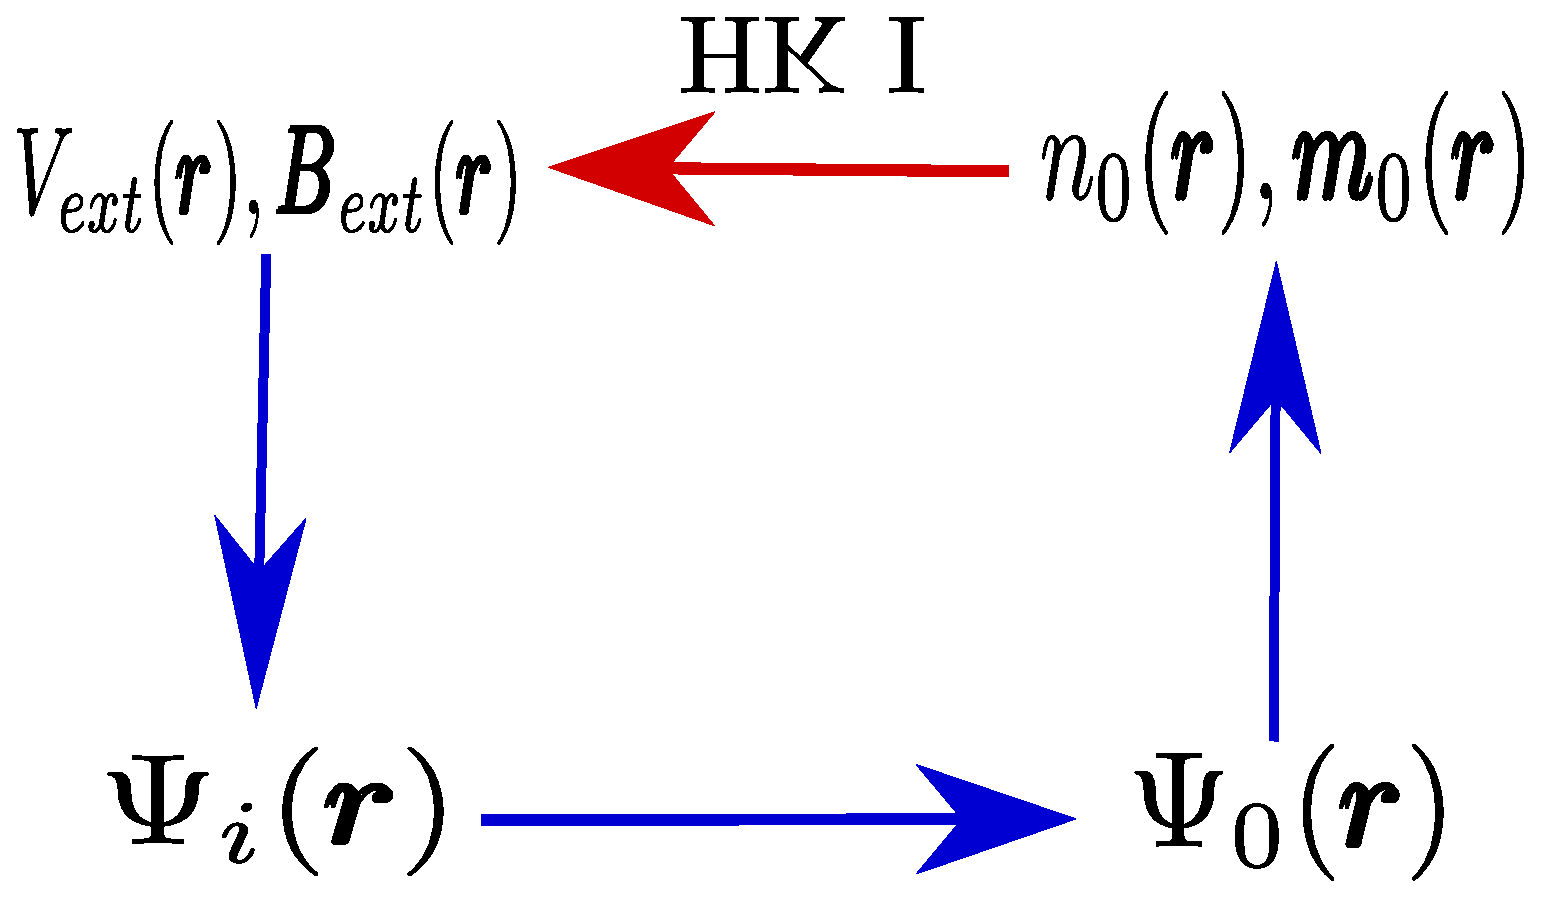
\epsfig{file=figuras/HK1.eps, width=8.0cm,height=5.0cm}
   		\caption{Representaci\'on esquem\'atica del primer teorema de Hohenberg-Kohn}
   		\label{fig:hk1}
   	\end{figure}
   }
  \frame{\frametitle{segundo teorema de Hohenberg-Kohn}
  	\begin{itemize}
  		\item se puede definir el funcional para la energ\'ia:
  		\begin{equation}
  		E_{V_{ext}, \pmb{B}_{ext}}[n,\pmb{m}]= F[n,\pmb{m}] + \int d \pmb{r} \{V_{ext} (\pmb{r}) n(\pmb{r})+\pmb{B}_{ext} (\pmb{r}) \pmb{m} (\pmb{r}) \} +E_{II} \label{ec:funcional}
  		\end{equation}
  		con
  		\begin{eqnarray}
  		F[n,\pmb{m}]&= \langle \Psi_0 [n,\pmb{m}]| \hat{T}+\hat{V}_{int} | \Psi_0 [n,\pmb{m}] \rangle \nonumber \\
  		&= T[n,\pmb{m}] + V_{int} [n,\pmb{m}] \label{ec:funcF}
  		\end{eqnarray}
  		
  	\end{itemize}
  }
  \frame{\frametitle{segundo teorema de Hohenberg-Kohn}
  	\begin{itemize}
  		\item en el estado base se cumple lo siguiente:
  		\begin{equation}
  		E_0 = \min_{n  \to n_0, \pmb{m} \to \pmb{m}_0} E_{V_{ext}, \pmb{B}_{ext}}[n,\pmb{m}]  \label{ec:HKII}
  		\end{equation}
  	\end{itemize}
  }
  \section{Ecuaciones de Kohn-Sham}
  \frame{\frametitle{Sistema auxiliar e kohn-Sham}
  	\begin{itemize}
  		\item se comienza con el Hamiltoniano auxiliar:
  		\begin{equation}
  		\hat{H}_{aux}^{s} = - \frac{1}{2} \nabla^2 + V_{eff}^s (\pmb{r}) \label{ec:HAux}
  		\end{equation} 
  		\pause
  		\item en un caso colineal con la densidad electr\'onica dada por:
  		\begin{equation}
  		n_s (\pmb{r}) = \sum_{i} n_{i,s} |\psi_{i,s } (\pmb{r})|^2 \label{ec:den1spin}
  		\end{equation}
  	\end{itemize}
  }
  \frame{\frametitle{Funcional de la energ\'ia}
  	\begin{equation}
  	E_{KS}[n] = T_{sp}[n]+ \int d \pmb{r} V_{ext} (\pmb{r}) n_s (\pmb{r}) +E_{Hartree} [n] + E_{XC}^s [n] + E_{II} \label{ec:funcHK}
  	\end{equation}
  	\pause
  	con la energ\'ia cin\'etica de una sola part\'icula $T_sp$ definida  como:
  	\begin{multline}
  	T_{sp} = -\frac{1}{2} \sum_{s} \sum_{i} n_{i,s} \int d^3 r ~\psi_{i,s }^* (\pmb{r}) \nabla^2 \psi_{i,s } (\pmb{r}) \\ = \frac{1}{2} \sum_{s} \sum_{i} n_{i,s} \int d^3 r  |\nabla \psi_{i,s } (\pmb{r}) |^2 \label{ec:funCinetica}
  	\end{multline}
  }
  \frame{\frametitle{Funcional de la energ\'ia}
  	y el funcional de intercambio y correlaci\'on:
  	\begin{multline}
  	E_{XC}^s [n] = F[n]-(T_{sp} [n]+E_{Hartree}[n])\\
  	= \langle \hat{T} \rangle - T_{sp} [n]+\langle \hat{V}_{int} \rangle-E_{Hartree} [n] \label{ec:eXC2}
  	\end{multline}
  }
  \frame{\frametitle{minimizaci\'on de la energ\'ia}
  	Para cumplir con el segundo teorema de Hohenberg y Kohn se minimiza el funcional de la energ\'ia (ec. \ref{ec:funcHK}) con respecto  a las funciones de los orbitales $\psi_{i,s } $: 
  	\begin{equation}
  	\frac{\delta E_{KS} [n_s]}{\delta \psi_{i,s } ^* (\pmb{r})}= \frac{\delta T_{sp} }{\delta \psi_{i,s } ^* (\pmb{r}) } + \left[\frac{\delta E_{ext}}{\delta n_s (\pmb{r})}+\frac{\delta E_{Hartree}}{\delta n_s (\pmb{r})}+  \frac{\delta E_{XC}^s}{\delta n_s (\pmb{r})}\right] \frac{\delta n_s (\pmb{r})}{\delta \psi_{i,s } ^* (\pmb{r})} =0 \label{ec:ecEulerFun}
  	\end{equation}
  }
  \frame{\frametitle{minimizaci\'on de la energ\'ia} 
  	\begin{itemize}
  		\item 
  		\begin{equation}
  		\frac{\delta T_{sp} }{\delta \psi_{i,s } ^* (\pmb{r}) }= -\frac{1}{2} \nabla^2 \psi_{i,s } (\pmb{r}); ~~ \frac{\delta n_s (\pmb{r})}{\delta \psi_{i,s } ^* (\pmb{r})}= \psi_{i,s } (\pmb{r}) \label{ec:simp}
  		\end{equation}
  		
  		
  		
  	\end{itemize}
  	
  }
  \frame{\frametitle{Ecuaciones de Kohn-Sham}
  	\begin{itemize}
  		\item 
  		\begin{equation}
  		(H_{KS}^s -\epsilon_{i,s})\psi_{i,s } (\pmb{r}) = 0 \label{ec:ShKS}
  		\end{equation}
  		\pause
  		\item con el el hamiltoniano efectivo definido por:
  		\begin{equation}
  		H_{KS}^s = -\frac{1}{2} \nabla^2 + V_{KS}^s (\pmb{r}) \label{ec:HamiltonianoKS}
  		\end{equation}
  		\pause
  		\item y el potencial:
  		\begin{eqnarray}
  		V_{KS}^s (\pmb{r}) &=& V_{ext} (\pmb{r})+  \frac{\delta E_{Hartree}}{\delta n_s (\pmb{r})}+  \frac{\delta E_{XC}^s}{\delta n_s (\pmb{r})} \nonumber \\
  		&=& V_{ext} (\pmb{r})+ V_{Hartree} (\pmb{r}) + V_{XC}^s (\pmb{r}) \label{ec:potKS} 
  		\end{eqnarray}
  	\end{itemize}
  }
  \frame{
  	\begin{figure}[!hbt]
  		\centering
  		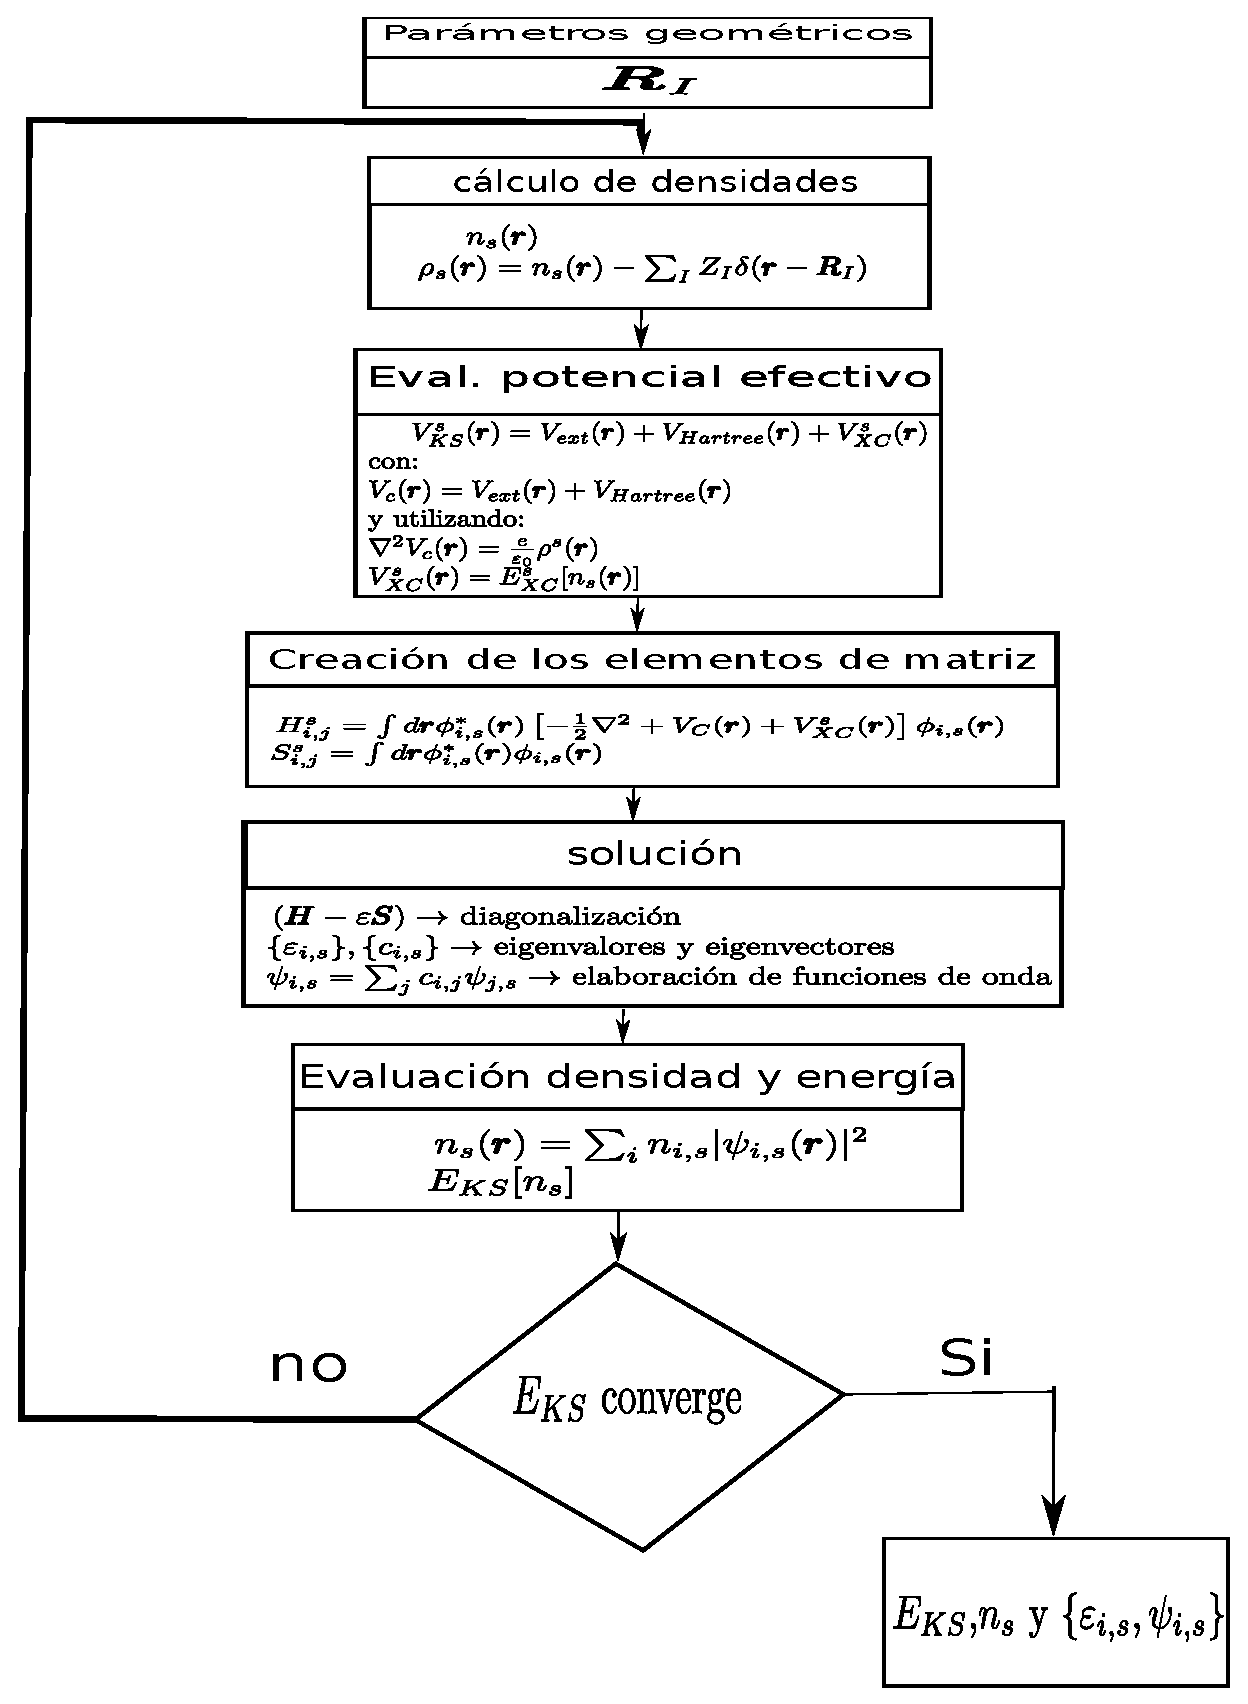
\epsfig{file=figuras/diagramaAuto.eps, width=4.0cm,height=8.0cm}
  		
  		\label{fig:esq}
  	\end{figure}
  }
  \frame{\frametitle{caso no colineal}
  	\begin{itemize}
  		\item Se tiene que agregar el siguiente t\'ermino
  		\begin{equation*}
  		B_{XCj} (\pmb{r}) = - \frac{\delta E_{XC} [n,\pmb{m}]}{\delta m_j (\pmb{r})}
  		\end{equation*}
  		\pause
  		\item La ecuaci\'on a resolver es:
  		\begin{multline}
  		\sum_{s}  \left[-\frac{1}{2} \nabla^2 + V_{ext} (\pmb{r})+ V_{Hartree} (\pmb{r}) + V_{XC} (\pmb{r}) \right] \delta_{s',s}  \phi_{\Lambda} (\pmb{r},s)\\ - \mu_{B} \sum_{s}  [\pmb{B}_{ext} (\pmb{r})+ \pmb{B}_{XC} (\pmb{r}) ] \pmb{\sigma_{s,s'}} \phi_{\Lambda} (\pmb{r},s) = \varepsilon_{\Lambda} \phi_{\Lambda} (\pmb{r},s) \label{ec:KSnoColl}
  		\end{multline}
  	\end{itemize}
  }
 \frame{\frametitle{Funcional de Harris}
 	\begin{multline}
 	E_{Harris} [n_0] = \sum_{i} \varepsilon_i - \int d^3 r V_{ext} [n_0] n_0 (\pmb{r}) \\ - \frac{1}{2} \int d^3 r V_{Hartree} [n_0] n_0 (\pmb{r}) + E_{XC} [n_0] \label{ec:FuncHarris}
 	\end{multline}
 }
\section{funcional PBE}
  \frame{
  	\frametitle{funcional de gradientes generalizados}
  	El funcional de intercambio y correlaci\'on puede tomar la siguiente forma:
  	\begin{multline}
  	E_{XC}^{GGA} [n_{\uparrow} (\pmb{r}), n_{\downarrow}(\pmb{r})] = \int d^3 r ~ n(\pmb{r}) \epsilon_{XC} \left(n_{\uparrow} (\pmb{r}), n_{\downarrow}(\pmb{r}), \left|\nabla n_{\uparrow} (\pmb{r}) \right|^2, \left|\nabla n_{\downarrow} (\pmb{r}) \right|^2 \right)  \\
  	= \int d^3 r ~ n(\pmb{r}) \epsilon_{X}^{hom} (n) F_{XC} \left(n_{\uparrow} (\pmb{r}), n_{\downarrow}(\pmb{r}), \left|\nabla n_{\uparrow} (\pmb{r}) \right|^2, \left|\nabla n_{\downarrow} (\pmb{r}) \right|^2 \right) \label{ec:funcXCGGA}
  	\end{multline}
  	en donde $ \epsilon_{X}^{hom} (n) = -3k_F / 4\pi $ es la energ\'ia de intercambio pro part\'icula  de un gas de electrones homog\'eneo no polarizado en donde $k_F = (3 \pi^2 n)^{1/3}$ es el vector de onda de Fermi.
  }
 \frame{\frametitle{Funcional PBE}
 	\begin{itemize}
 		\item El funcional de intercambio y  correlaci\'on se divide en:
 		\begin{equation*}
 		\epsilon_{XC} (\pmb{r}; [n] )= \epsilon_{X} (\pmb{r}; [n] )+ \epsilon_{C} (\pmb{r}; [n] )
 		\end{equation*}
 		\pause
 		\item El funcional e intercambio:
 		\begin{equation}
 		E_X [n_{\uparrow}, n_{\downarrow}]= \frac{1}{2} \left[E_{X} [2 n_{\uparrow}] + E_{X} [2 n_{\downarrow}]   \right] \label{ec:divEx}
 		\end{equation}
 		y utiliando el gradiente de densidad reducida:
 		\begin{equation}
 		s(\pmb{r})= \frac{|\nabla n (\pmb{r})|}{2 k_F n (\pmb{r}) } \label{ec:S}
 		\end{equation}
 		
 	\end{itemize}
 }
 \frame{\frametitle{Funcional PBE}
 	\begin{itemize}
 		\item Se puede escribir $F_X (s)$ :
 		\begin{equation}
 		F_{X}^{PBE} = 1+\kappa -\frac{\kappa}{1+\mu s^2 /\kappa} \label{ec:F_X-PBE}
 		\end{equation}
 		donde $\mu = 0.21951 $ y $\kappa= 0.804 $.
 		\pause
 		\item la energ\'ia de correlaci\'on":
 		\begin{equation}
 		E_{C} ^{PBE} = \int d^3 r n \left\{\epsilon_{C}(r_s,\zeta)+ H^{PBE} (r_s,\zeta,t) \right\}\label{ec:funcCorr}
 		\end{equation}
 		donde $r_s = (3/4 \pi n)^{1/3}, ~ \zeta =(n_{\uparrow}-n_{\downarrow})/n, t=|\nabla n|/2 k_s \phi n, \phi= \frac{1}{2} [(1+\zeta)^{2/3}+(1-\zeta)^{2/3}], k_s = (4 k_F/\pi)^{1/2}$,
 		\begin{equation}
 		H^{PBE} = \gamma \phi^3 \ln \left\{1+ \frac{\beta}{\gamma} t^2 \left[\frac{1+At^2}{1+At^2+A^2 t^4}\right]\right\}, \label{ec:PBEH}
 		\end{equation}
 		\begin{equation}
 		A=\frac{\beta}{\gamma} [exp\{-\epsilon_{C}^{hom}/\gamma \phi^3 \}-1]^{-1} \label{ec:A}
 		\end{equation}
 		y $\gamma=0.031091, ~\beta=0.066725$.
 		
 	\end{itemize}
 }
\frame{\frametitle{potencial de intercambio y correlaci\'on}
	Este potencial est\'a dado por:
	\begin{equation}
	V_{XC}^s (\pmb{r}_m) = \left[\epsilon_{XC}+n \frac{\partial \epsilon_{XC}}{\partial n}\right]_{\pmb{r}_m, s} + \sum_{s'} \left[ n \frac{\partial \epsilon_{XC}}{\partial |\nabla n|} ~\frac{\nabla n}{\partial |\nabla n|}\right] _{\pmb{r}_m', s} \pmb{C}_{m'-m} \label{ec:potVxc}
	\end{equation}
	donde $\pmb{C}_{m} = \{ C_m ^x , C_m ^y , C_m ^z  \}$  es un vector en las coordenadas espaciales.
}
\section{formalismo en el espacio K}
\frame{\frametitle{ecuaciones de Kohn-Sham en el espacio rec\'iproco}
	\begin{itemize}
		\item se utiliza una base de ondas planas:
		\begin{equation}
		\phi_{\pmb{k},\pmb{G}} (\pmb{r})= \frac{1}{\sqrt{\Omega}} e^{i (\pmb{k}+\pmb{G})\pmb{r}} \label{ec:ondaplana}
		\end{equation}
		\pause
		\item Para un sistema translacionalmente invariante cada eigenfunci\'on de Kohn-Sham $\psi_{v,\pmb{k},s }$ que cumple con el teorema de Bloch se puede expandir como:
		\begin{equation}
		\psi_{v,\pmb{k},s } (\pmb{r}) = \sum_{\pmb{G}} c_{v,\pmb{k},s } \phi_{\pmb{k},\pmb{G}} (\pmb{r}) \label{ec:basePW}
		\end{equation}
		\pause
		\item la densidad se expresa como:
		\begin{eqnarray}
		n_s(\pmb{r}) &=& \sum_{\pmb{G}} e^{-i \pmb{G} \pmb{r}} \tilde{n}_s (\pmb{G})  \label{ec:desnsiadK}\\
		\tilde{n}_s (\pmb{G}) &=& \frac{1}{\Omega} \sum_{v,\pmb{k}} n_{v,\pmb{k},s} \sum_{\pmb{G'}} c_{v,\pmb{k},s}^* (\pmb{G'}+\pmb{G}) c_{v,\pmb{k},s} (\pmb{G'}) \nonumber
		\end{eqnarray}
	\end{itemize}
}
\frame{\frametitle{ecuaciones de Kohn-Sham en el espacio rec\'iproco}
	y la ecuaciones de Kohn-Sham \ref{ec:ShKS} toman la siguiente forma:
	\begin{equation}
	\sum_{\pmb{G'}} \left\{ \left[\frac{1}{2} (\pmb{k}+ \pmb{G})^2 - \varepsilon_{v,s} (\pmb{k}) \right] \delta_{\pmb{G},\pmb{G'}} + V_{KS} ^ s (\pmb{G}-\pmb{G'}) \right\} c_{v,\pmb{k},s} (\pmb{G'}) =0 \label{ec:HKSRes}
	\end{equation} 
}
\frame{
	\begin{figure}[!htb]
		\centering
		\subfigure[]
		{
			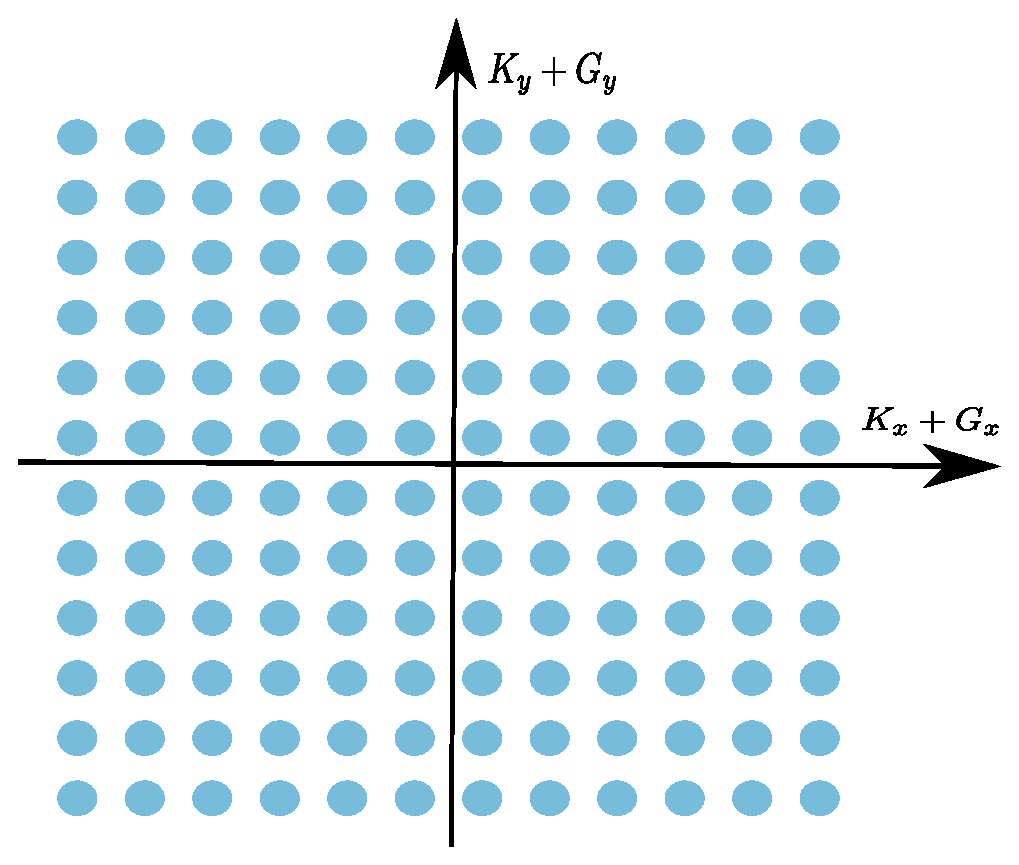
\epsfig{file=figuras/epacioKa.eps, width=5.0cm,height=5.0cm}
			\label{fig:a-espacioK}
		}
		\subfigure[]{
			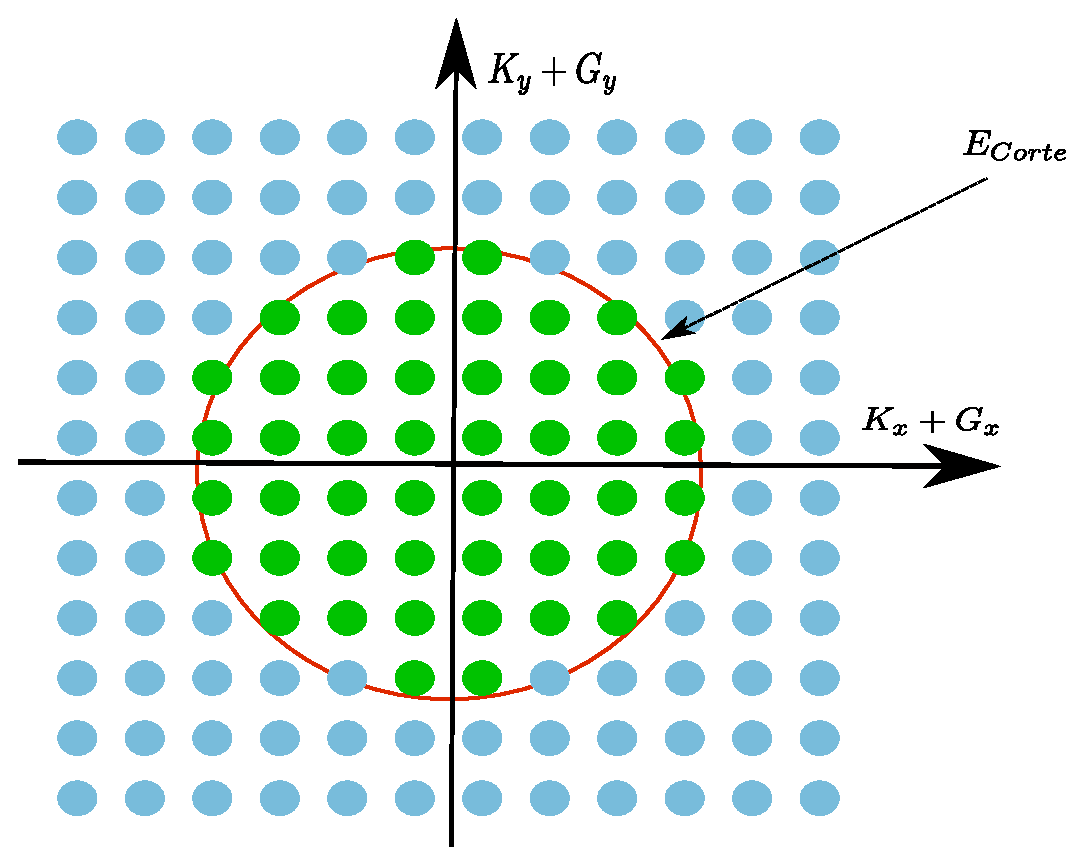
\epsfig{file=figuras/epacioKb.eps, width=5.0cm,height=5.0cm}
			\label{fig:b-espacioK}
		}
		\caption{en la figura \ref{fig:a-espacioK} se muestra el mapeo en el espacio rec\'iproco usando ondas planas. En la figura \ref{fig:b-espacioK} e muestra c\'omo  se trunca el espacio rec\'iproco por medio de la energ\'ia de corte $E_{corte} $}
		\label{fig:espacioK}
	\end{figure}
}
\frame{\frametitle{Energ\'ia de corte }
	En la pr\'actica el n\'umero de ondas planas es limitado a una energ\'ia de corte $E_{corte}$ relacionada con la energ\'ia cin\'etica:
	\begin{equation}
	\int d \pmb{r}  \phi_{\pmb{k},\pmb{G}}^* (\pmb{r}) \left\{-\frac{1}{2} \nabla^2 \right\} \phi_{\pmb{k},\pmb{G}} (\pmb{r}) = \frac{1}{2} (\pmb{k}+ \pmb{G})^2 \le E_{corte}. \label{ec:Ecut}
	\end{equation}
}
\frame{\frametitle{mapeo de  Monkhorst y Pack}
	\begin{equation}
	\pmb{k}_{n_1, n_2, n_3} = \sum_{i}^{3} \frac{2 n_i -N_i-1}{2N_i} \pmb{G}_i \label{ec:sampleMP}
	\end{equation}
	en donde $\pmb{G}_i $ son los vectores base del espacio rec\'iproco, $N_i$ es el n\'umero total de puntos en la direcci\'on $i$ y $n_i$ es el n]'umero de puntos \pmb{k} entre dos puntos en el espacio rec\'iproco conectados a trav\'es de  $\pmb{G}_i $.
}
\section{resultados strain}
\subsection{strain celdas unitarias}
\frame{\frametitle{strain isotr\'opico}
	$\varepsilon = \frac{a-a_1}{a_1} $
	\begin{figure}[!hbt]
		\centering
		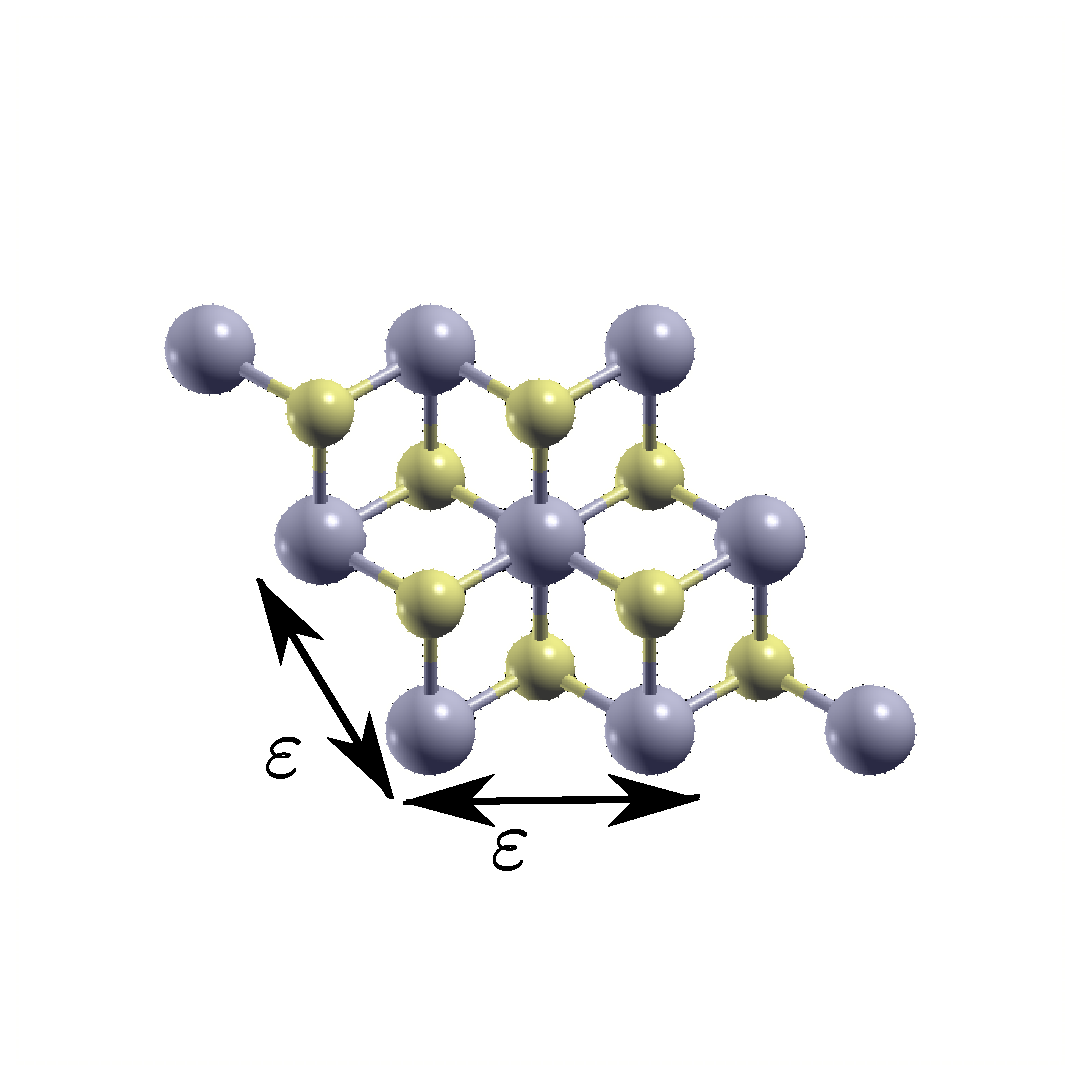
\epsfig{file=figRes/strainIso.eps, width=5.0cm,height=5.0cm}
		%\caption{Strain isotr\'opico}
		\label{fig:strIsoU}
	\end{figure}
}
\frame{\frametitle{distancias}
	\begin{figure}[!hbt]
		\centering
		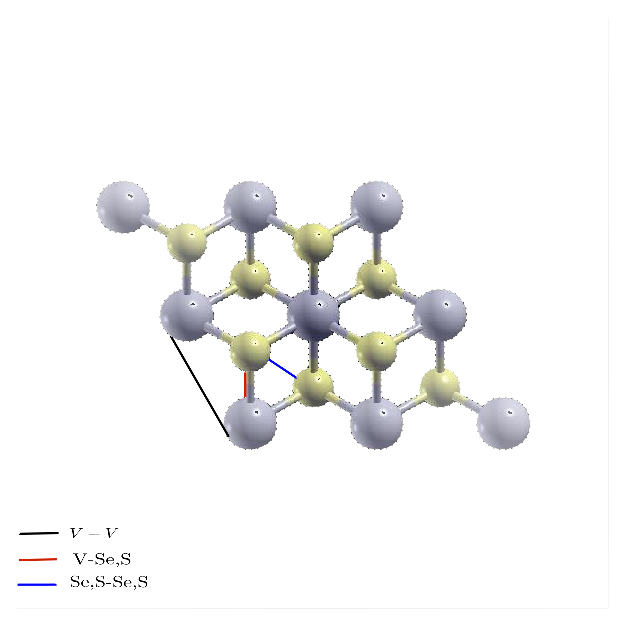
\epsfig{file=figRes/compIso.eps, width=7.0cm,height=7.0cm}
		%\caption{Strain isotr\'opico}
		\label{fig:strIsoUComp}
	\end{figure}
}
\frame{\frametitle{$VS_2$}
	\framesubtitle{magnetizaci\'on}
	
	\begin{figure}[!hbt]
		\centering
		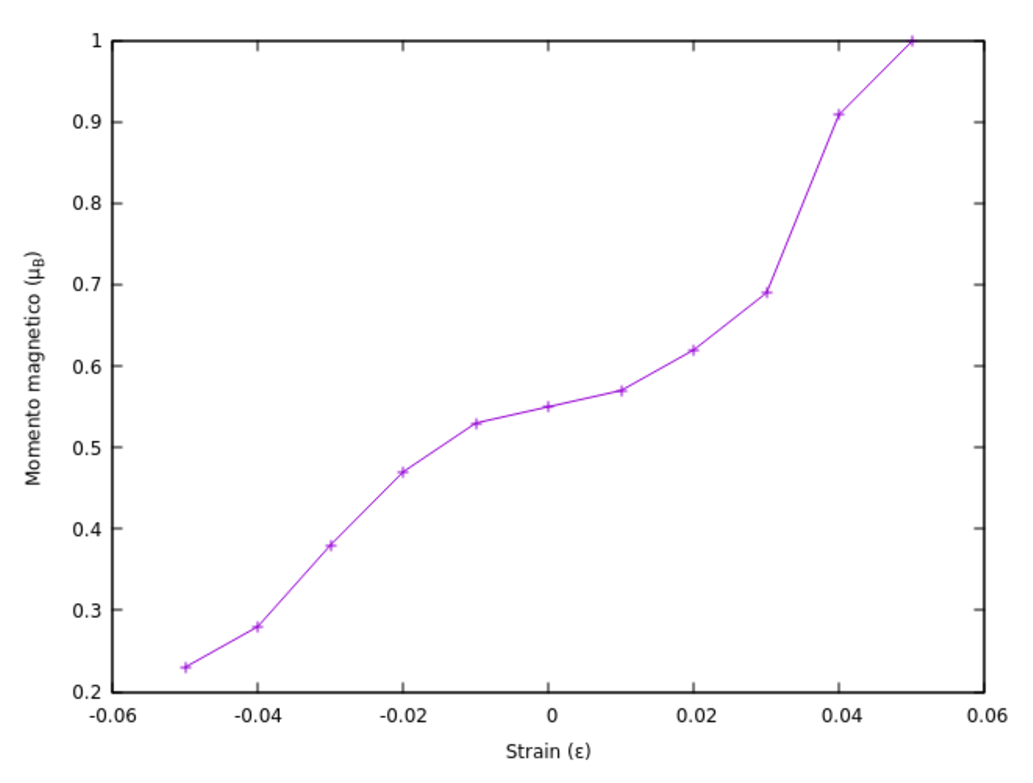
\epsfig{file=figRes/VS2/celdaU/strain/isotropico/mangVS2U.eps, width=7.0cm,height=7.0cm}
		%\caption{Strain isotr\'opico}
		\label{fig:VS2magn}
	\end{figure}

}
\frame{\frametitle{$VS_2$}
	\framesubtitle{$\Delta S $}
	
	\begin{figure}[!hbt]
		\centering
		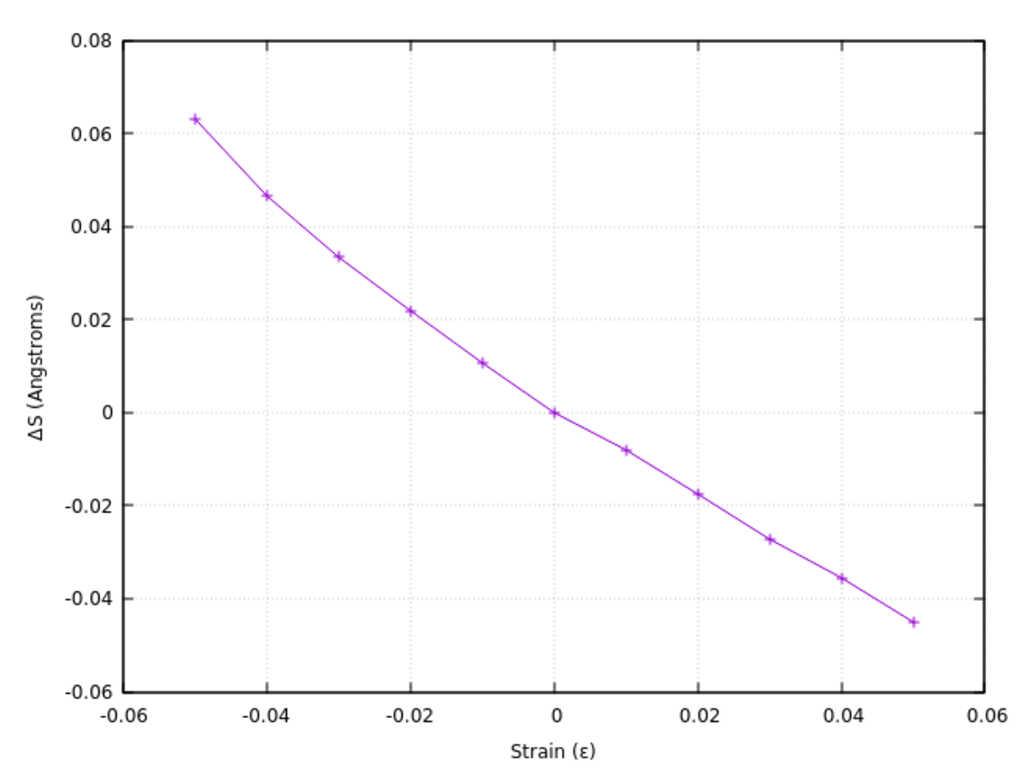
\epsfig{file=figRes/VS2/celdaU/strain/isotropico/deltaS.eps, width=7.0cm,height=7.0cm}
		%\caption{Strain isotr\'opico}
		\label{fig:dS1}
	\end{figure}
}

\frame{\frametitle{$VS_2$}
	\framesubtitle{$\Delta V-S $}
	
	\begin{figure}[!hbt]
		\centering
		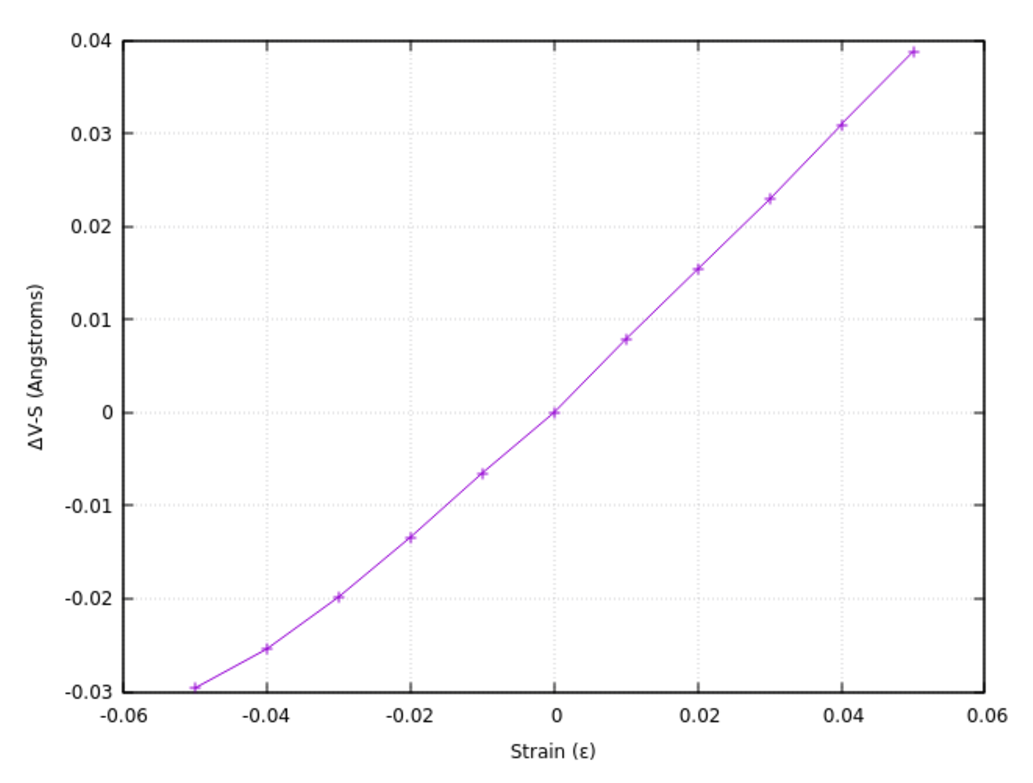
\epsfig{file=figRes/VS2/celdaU/strain/isotropico/deltaVsVS2U.eps, width=7.0cm,height=7.0cm}
		%\caption{Strain isotr\'opico}
		\label{fig:dSV1}
	\end{figure}
}
\frame{\frametitle{$VS_2$}
	\framesubtitle{$\Delta V $}
	
	\begin{figure}[!hbt]
		\centering
		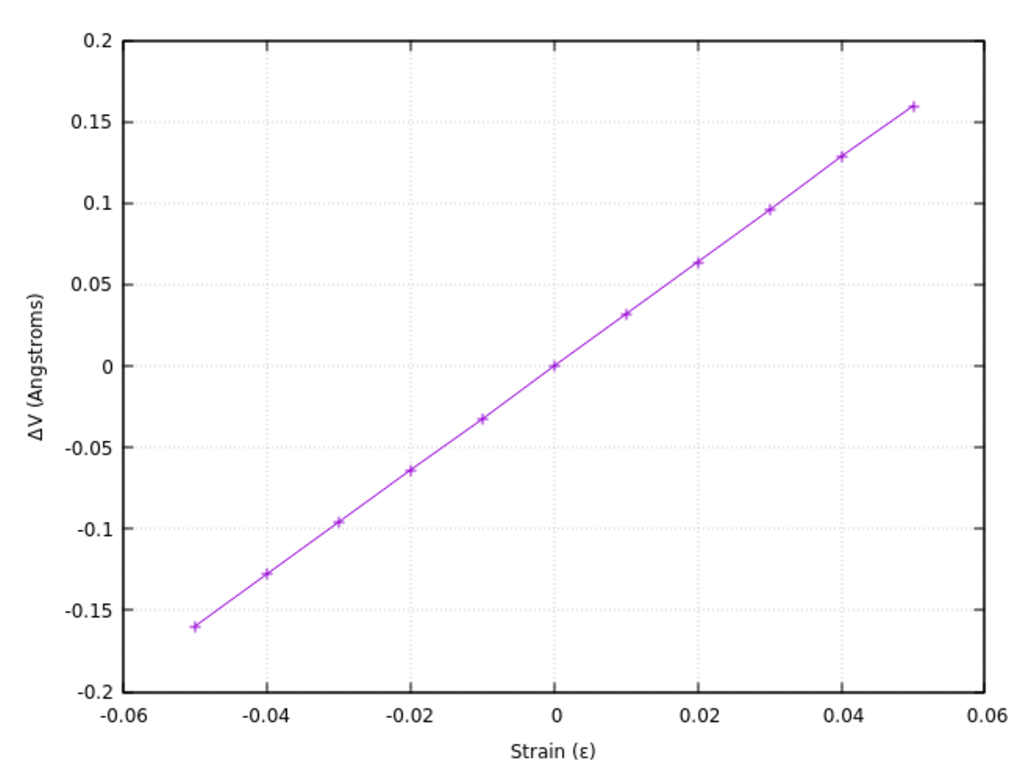
\epsfig{file=figRes/VS2/celdaU/strain/isotropico/deltaVVS2U.eps, width=7.0cm,height=7.0cm}
		%\caption{Strain isotr\'opico}
		\label{fig:dV1}
	\end{figure}
}


\frame{
	\frametitle{$PtSe_2 ~y ~PtS_2$}
	\framesubtitle{magnetizaci\'on}
	
	\begin{figure}[!hbt]
		\centering
		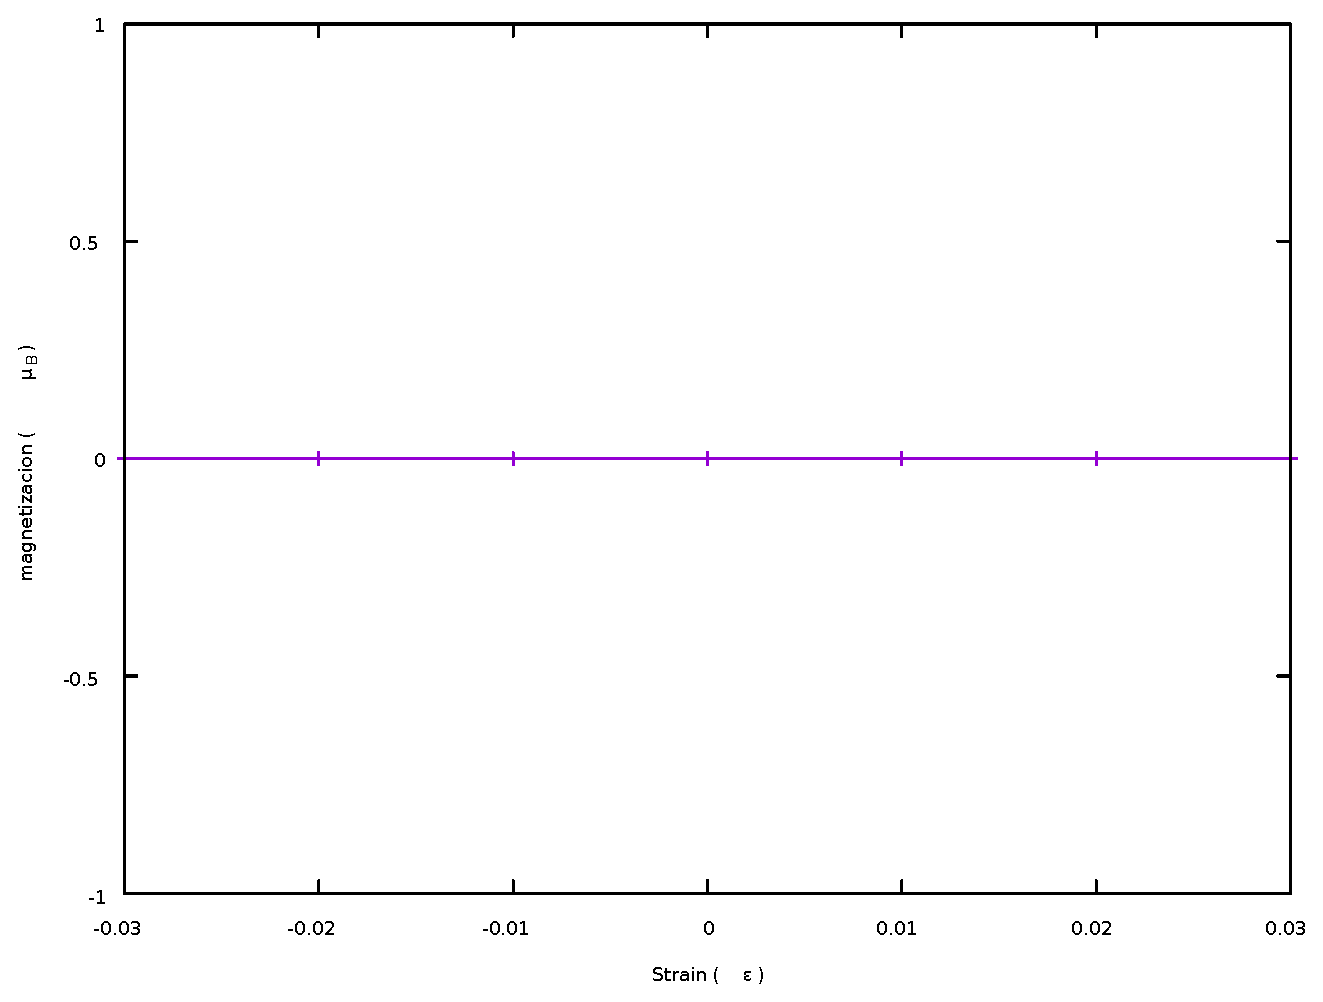
\epsfig{file=figRes/PtS2/iso/magn.eps, width=7.0cm,height=7.0cm}
		%\caption{Strain isotr\'opico}
		\label{fig:PtSe21}
	\end{figure}
}

\frame{\frametitle{$PtS_2$}
	\framesubtitle{$\Delta S $}
	
	\begin{figure}[!hbt]
		\centering
		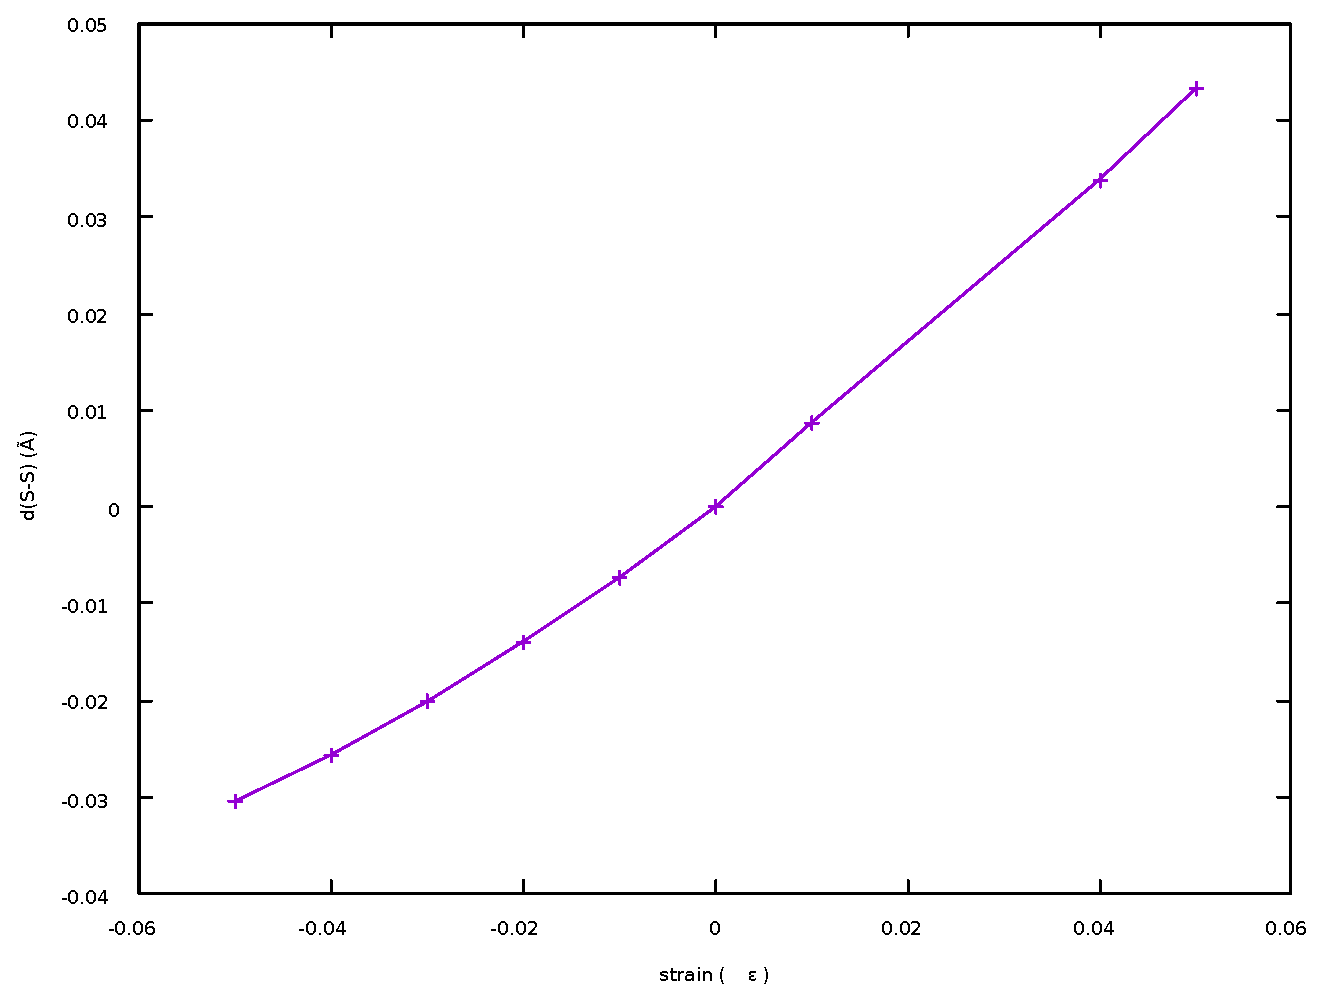
\epsfig{file=figRes/PtS2/iso/ds.eps, width=7.0cm,height=7.0cm}
		%\caption{Strain isotr\'opico}
		\label{fig:dS3}
	\end{figure}
}

\frame{\frametitle{$PtS_2$}
	\framesubtitle{$\Delta Pt-S $}
	
	\begin{figure}[!hbt]
		\centering
		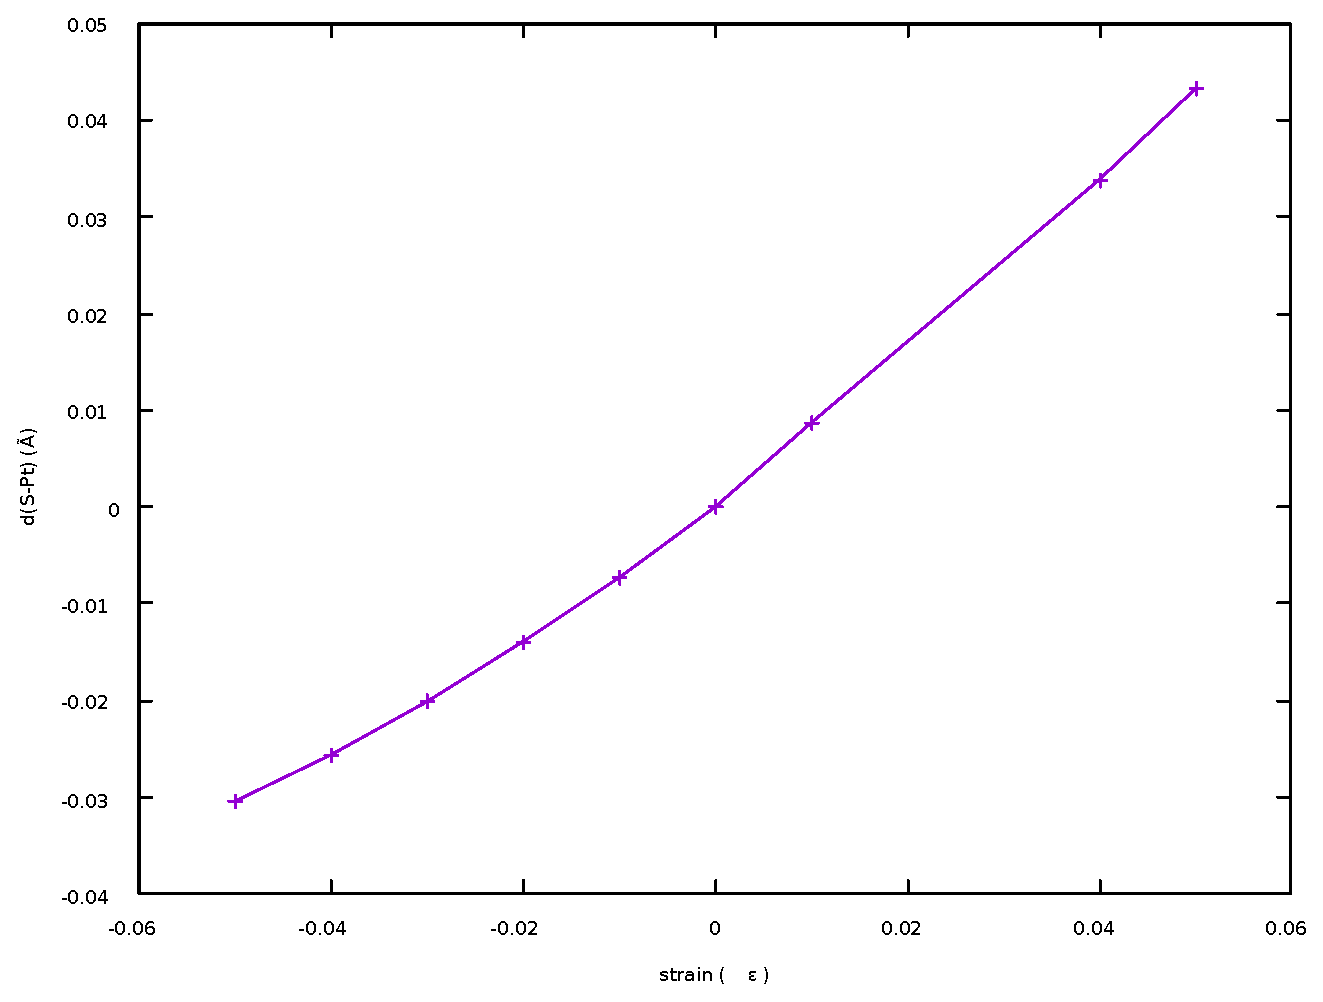
\epsfig{file=figRes/PtS2/iso/dPtS.eps, width=7.0cm,height=7.0cm}
		%\caption{Strain isotr\'opico}
		\label{fig:dSePt1}
	\end{figure}
}
\frame{\frametitle{$PtS_2$}
	\framesubtitle{$\Delta Pt $}
	
	\begin{figure}[!hbt]
		\centering
		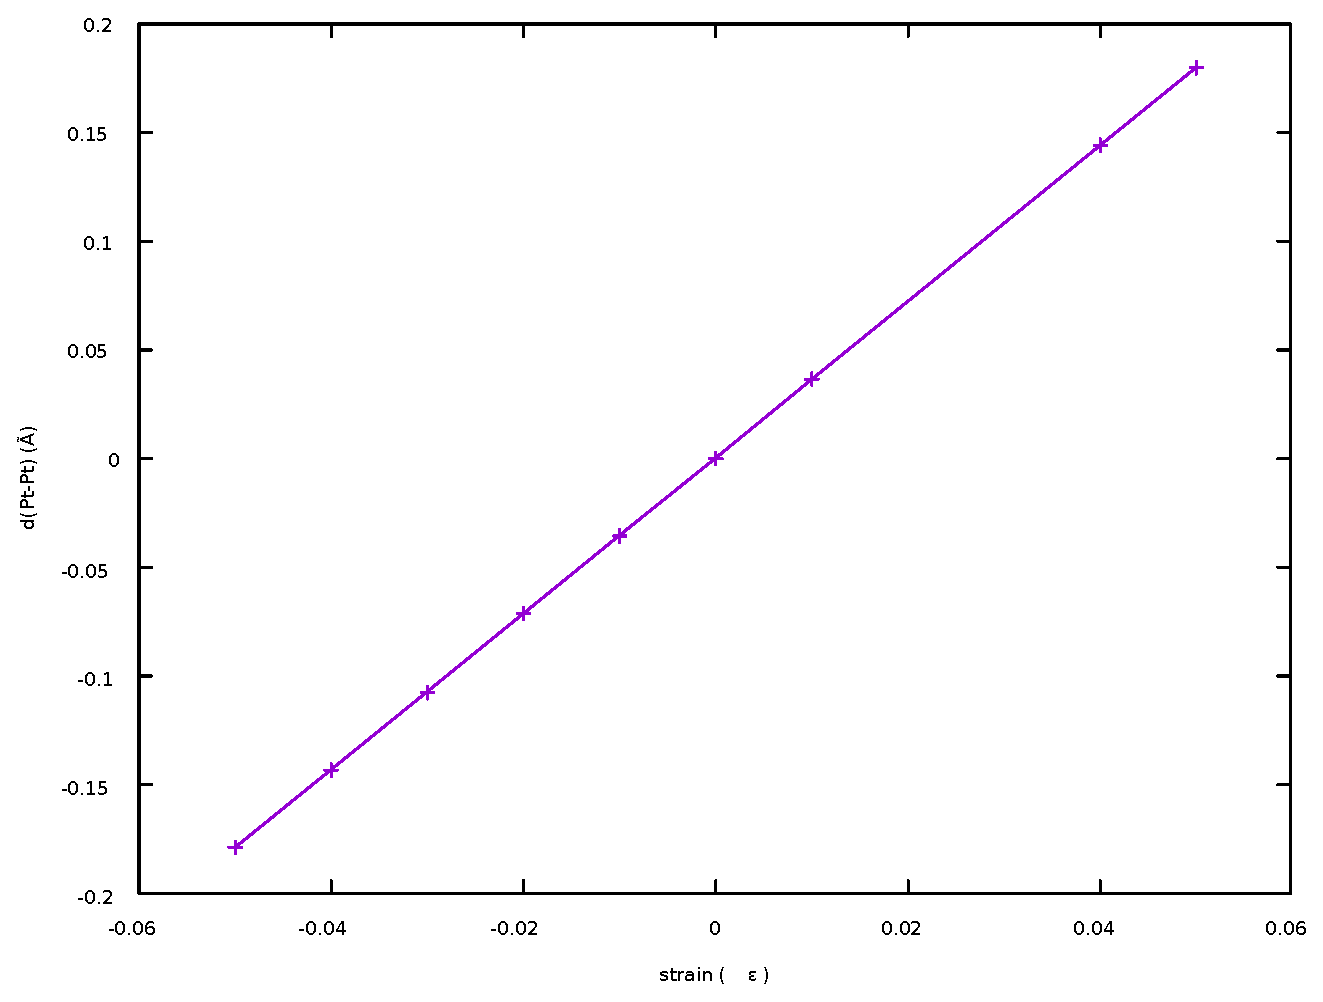
\epsfig{file=figRes/PtS2/iso/dPt.eps, width=7.0cm,height=7.0cm}
		%\caption{Strain isotr\'opico}
		\label{fig:dPt1}
	\end{figure}
}

\frame{\frametitle{$PtSe_2$}
	\framesubtitle{$\Delta Se $}
	
	\begin{figure}[!hbt]
		\centering
		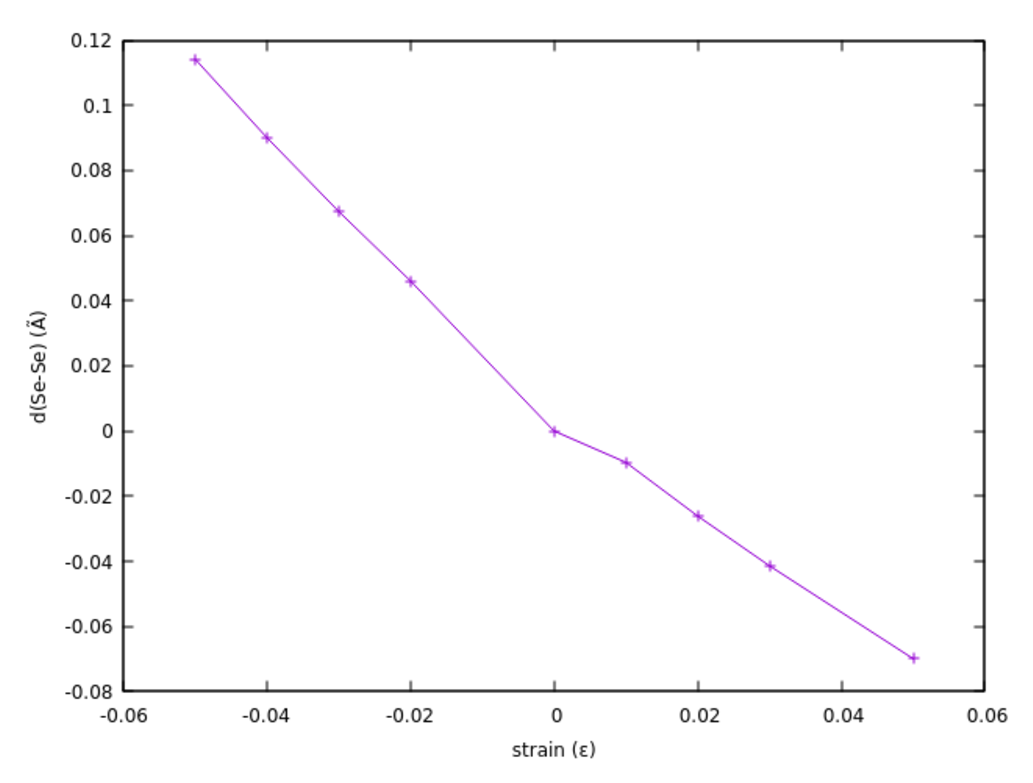
\epsfig{file=figRes/PtSe2/iso/dSS.eps, width=7.0cm,height=7.0cm}
		%\caption{Strain isotr\'opico}
		\label{fig:dSe3}
	\end{figure}
}

\frame{\frametitle{$PtSe_2$}
	\framesubtitle{$\Delta Pt-Se $}
	
	\begin{figure}[!hbt]
		\centering
		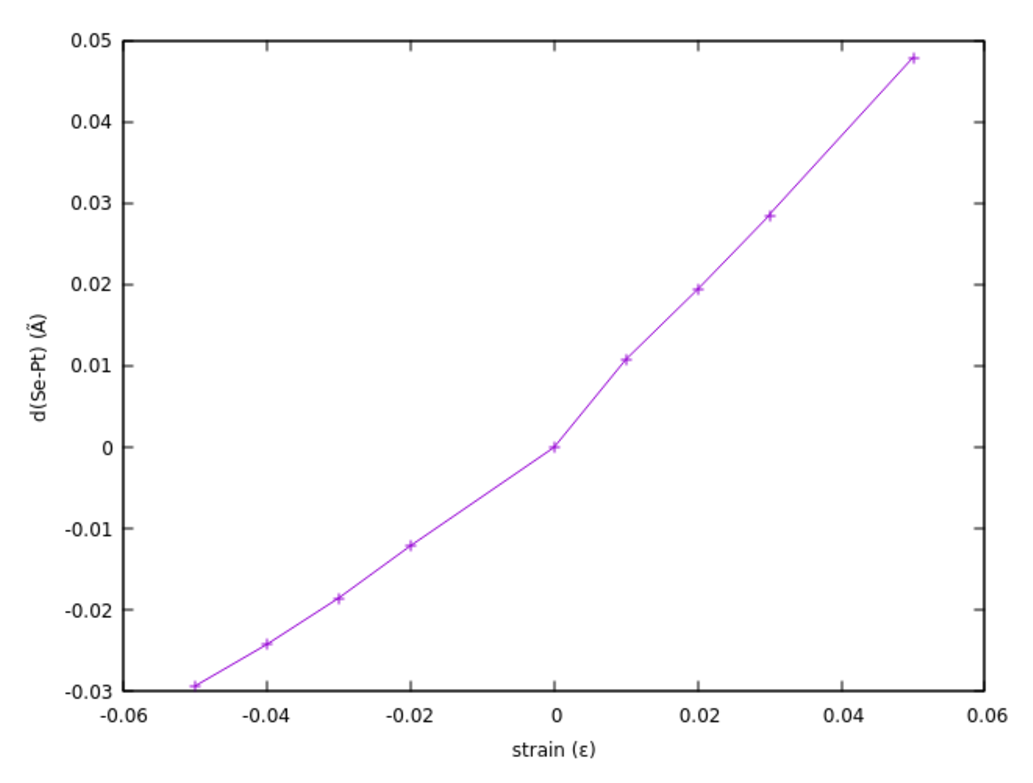
\epsfig{file=figRes/PtSe2/iso/dSPt.eps, width=7.0cm,height=7.0cm}
		%\caption{Strain isotr\'opico}
		\label{fig:dSPt1}
	\end{figure}
}
\frame{\frametitle{$PtSe_2$}
	\framesubtitle{$\Delta Pt $}
	
	\begin{figure}[!hbt]
		\centering
		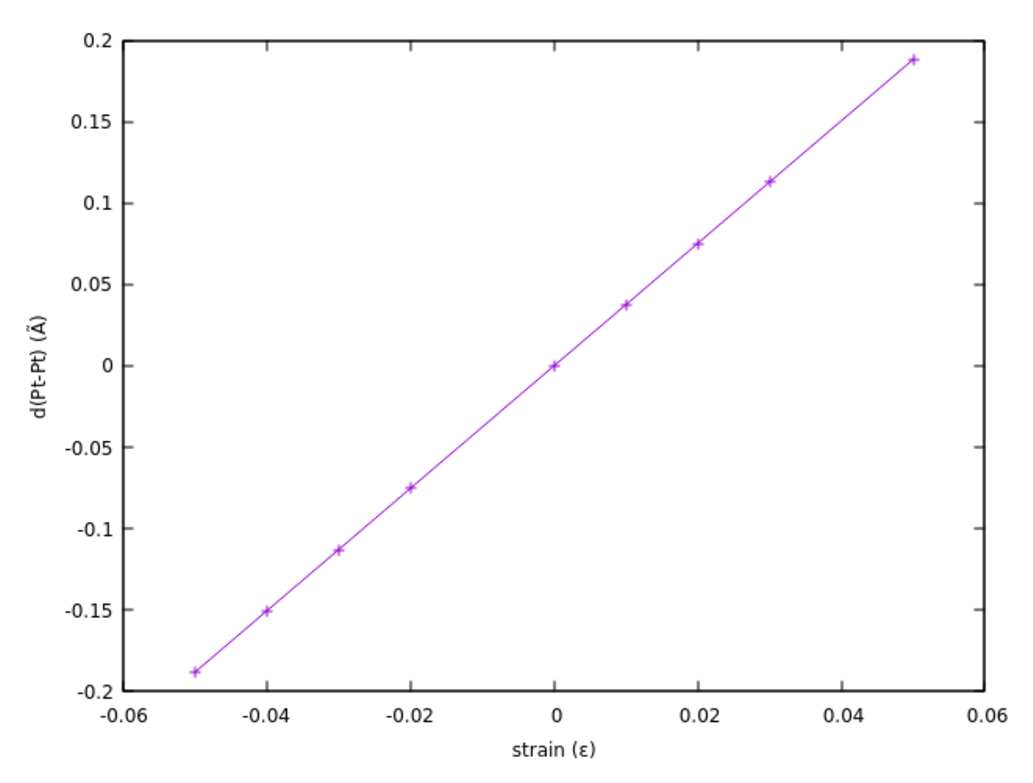
\epsfig{file=figRes/PtSe2/iso/dPt.eps, width=7.0cm,height=7.0cm}
		%\caption{Strain isotr\'opico}
		\label{fig:dPt2}
	\end{figure}
}

\frame{\frametitle{strain anisotr\'opico}
	$\varepsilon = \frac{a-a_1}{a_1} $
	\begin{figure}[!hbt]
		\centering
		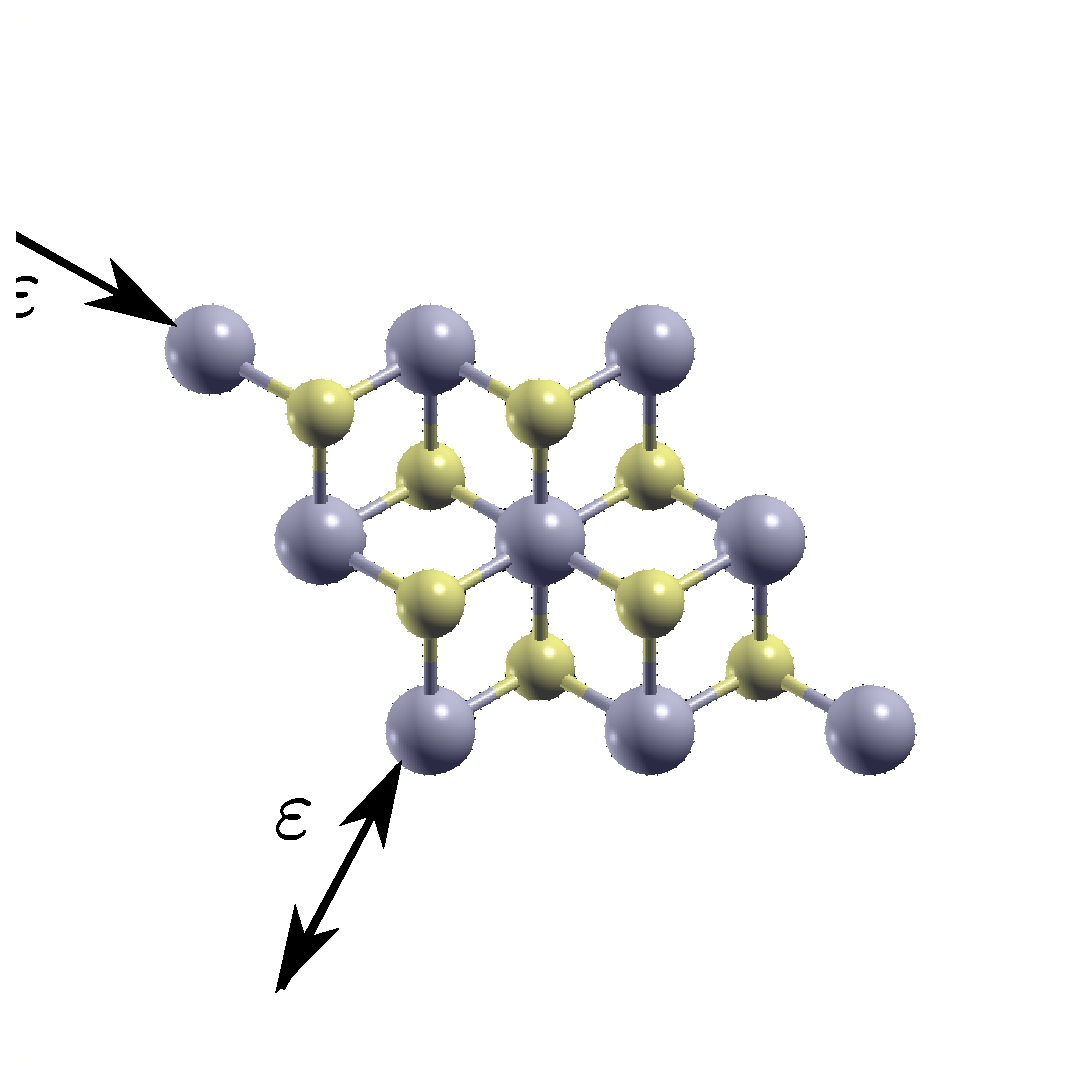
\epsfig{file=figRes/strainAnis.eps, width=5.0cm,height=5.0cm}
		%\caption{Strain isotr\'opico}
		\label{fig:strAnisU}
	\end{figure}
}
\frame{\frametitle{distancias}
	\begin{figure}[!hbt]
		\centering
		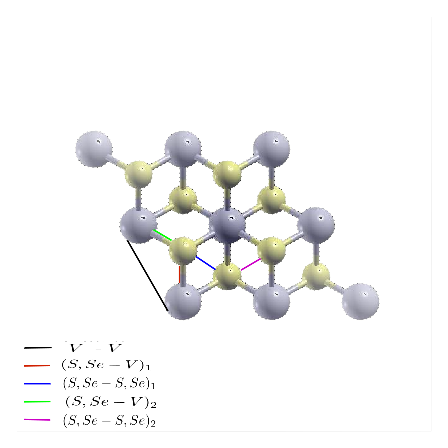
\epsfig{file=figRes/compAnis.eps, width=7.0cm,height=7.0cm}
		%\caption{Strain isotr\'opico}
		\label{fig:strAnisUComp}
	\end{figure}
}

\frame{\frametitle{$VS_2$}
	\framesubtitle{magnetizaci\'on}
	
	\begin{figure}[!hbt]
		\centering
		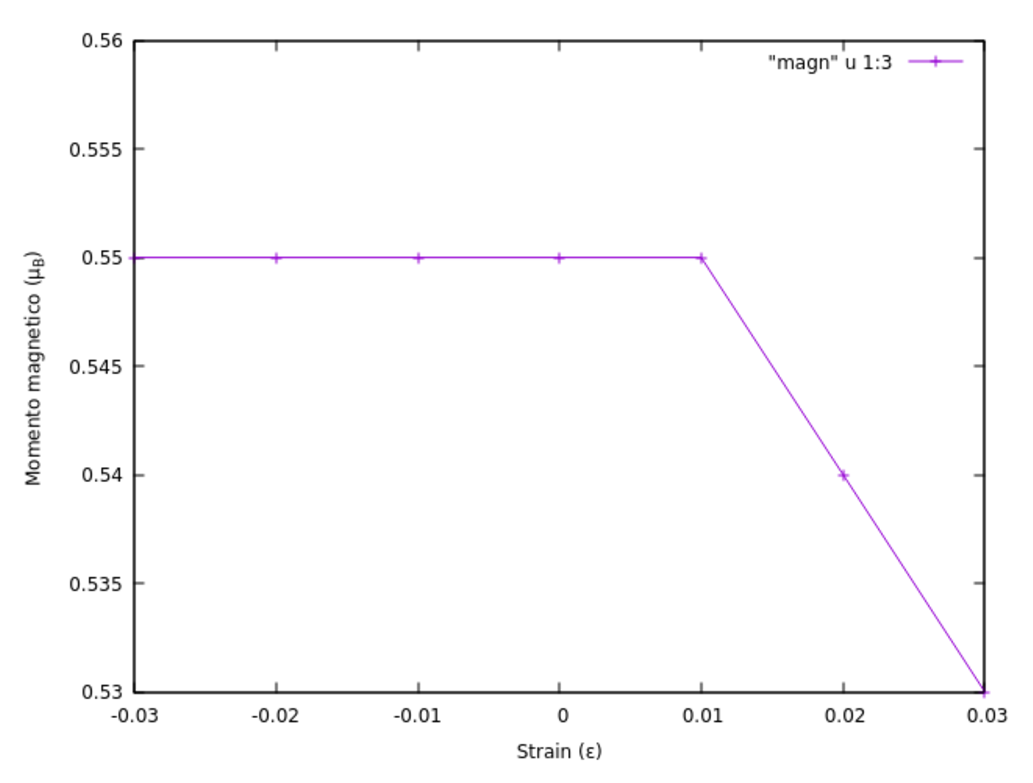
\epsfig{file=figRes/VS2/celdaU/strain/anisotropico2/MAGN.eps, width=7.0cm,height=7.0cm}
		%\caption{Strain isotr\'opico}
		\label{fig:VS2magna}
	\end{figure}
	
}
\frame{\frametitle{$VS_2$}
	\framesubtitle{comparativo $\Delta S $}
	
	\begin{figure}[!hbt]
		\centering
		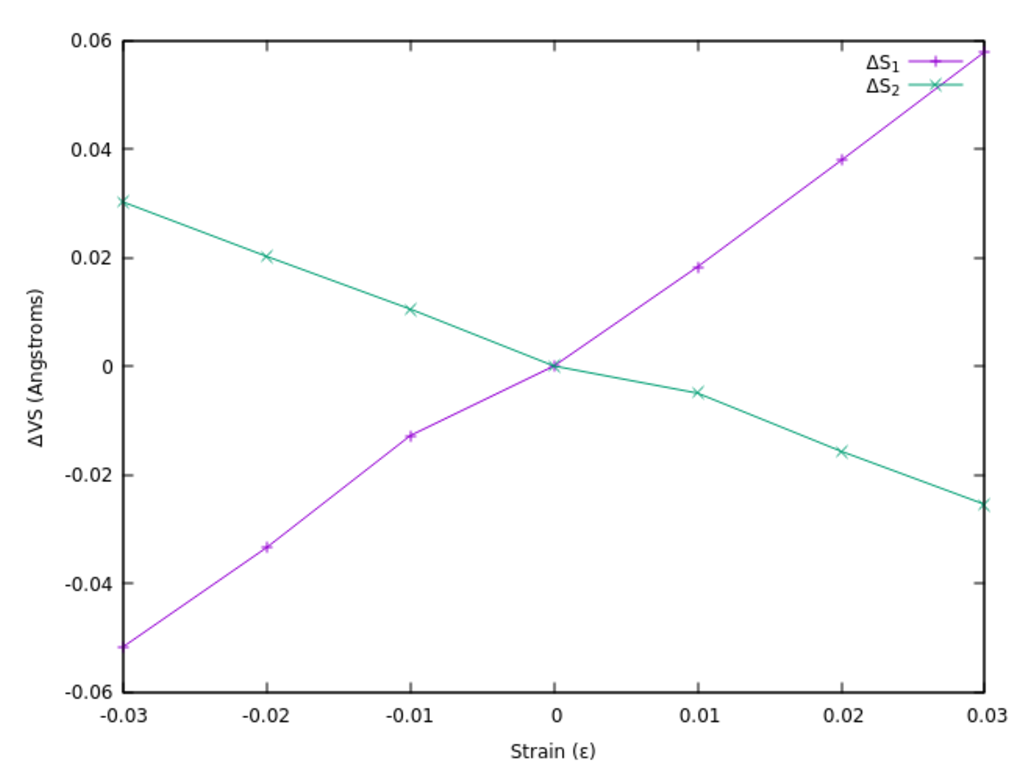
\epsfig{file=figRes/VS2/celdaU/strain/anisotropico2/compdeltaS.eps, width=7.0cm,height=7.0cm}
		%\caption{Strain isotr\'opico}
		\label{fig:CompdS}
	\end{figure}
}

\frame{\frametitle{$VS_2$}
	\framesubtitle{comparativo $\Delta V-S $}
	
	\begin{figure}[!hbt]
		\centering
		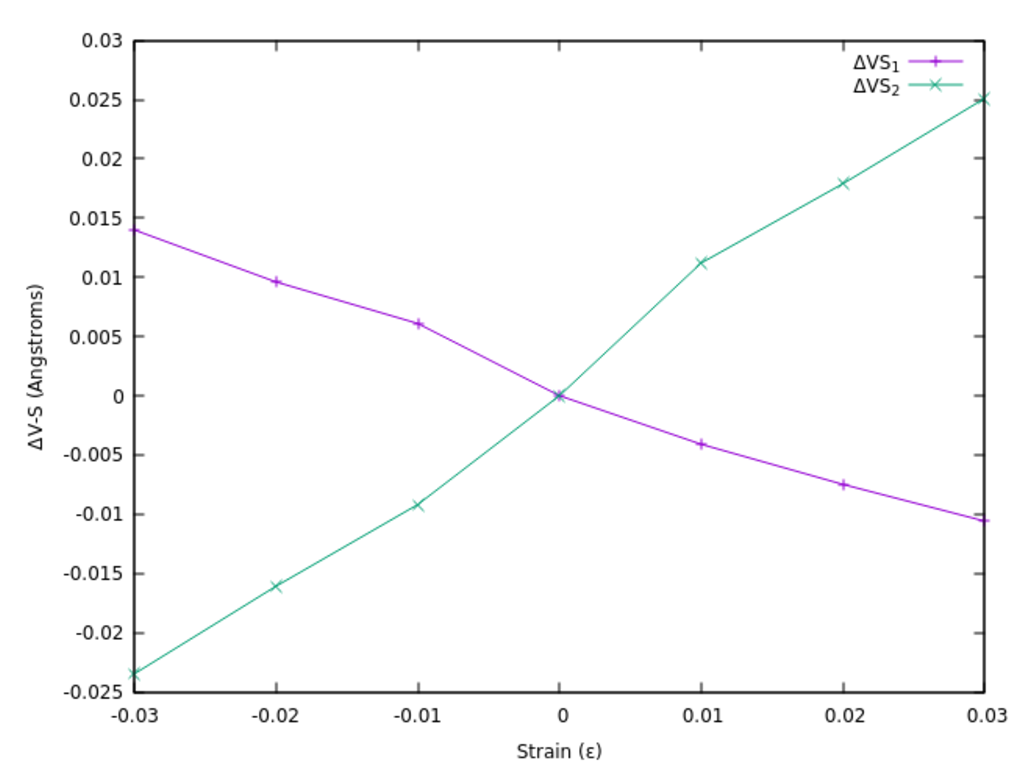
\epsfig{file=figRes/VS2/celdaU/strain/anisotropico2/deltavsComp.eps, width=7.0cm,height=7.0cm}
		%\caption{Strain isotr\'opico}
		\label{fig:compdSV}
	\end{figure}
}
\frame{\frametitle{$VS_2$}
	\framesubtitle{$\Delta V $}
	
	\begin{figure}[!hbt]
		\centering
		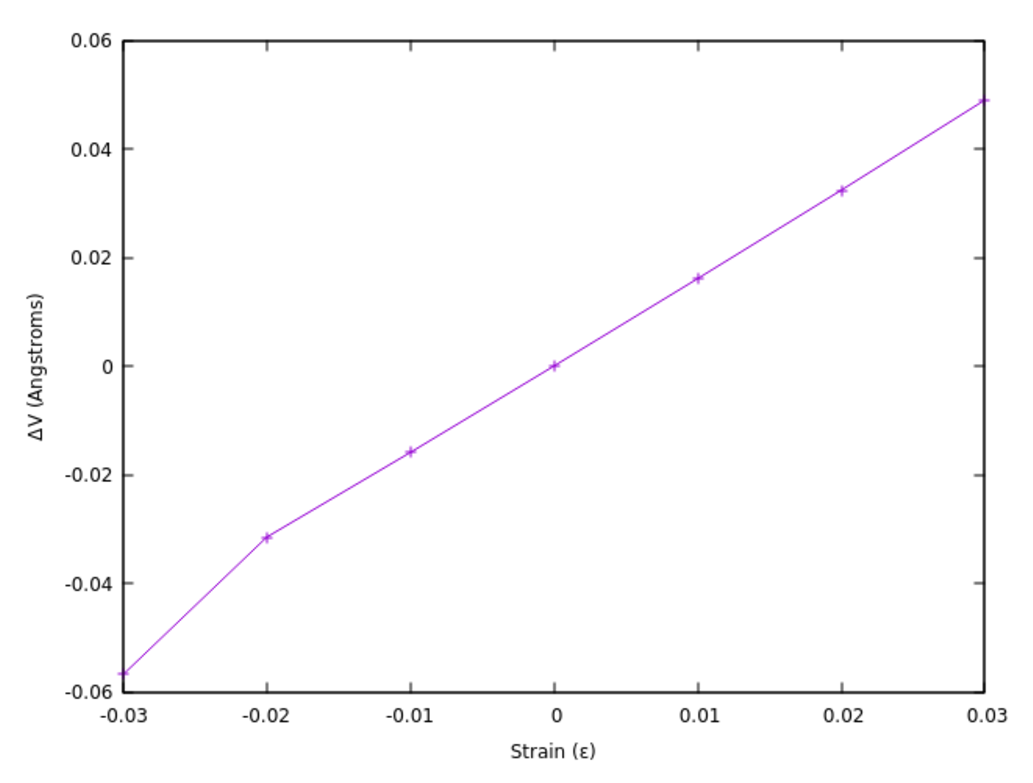
\epsfig{file=figRes/VS2/celdaU/strain/anisotropico2/deltaV.eps, width=7.0cm,height=7.0cm}
		%\caption{Strain isotr\'opico}
		\label{fig:dVa}
	\end{figure}
}

\frame{\frametitle{$PtS_2$}
	\framesubtitle{comparativo $\Delta S $}
	
	\begin{figure}[!hbt]
		\centering
		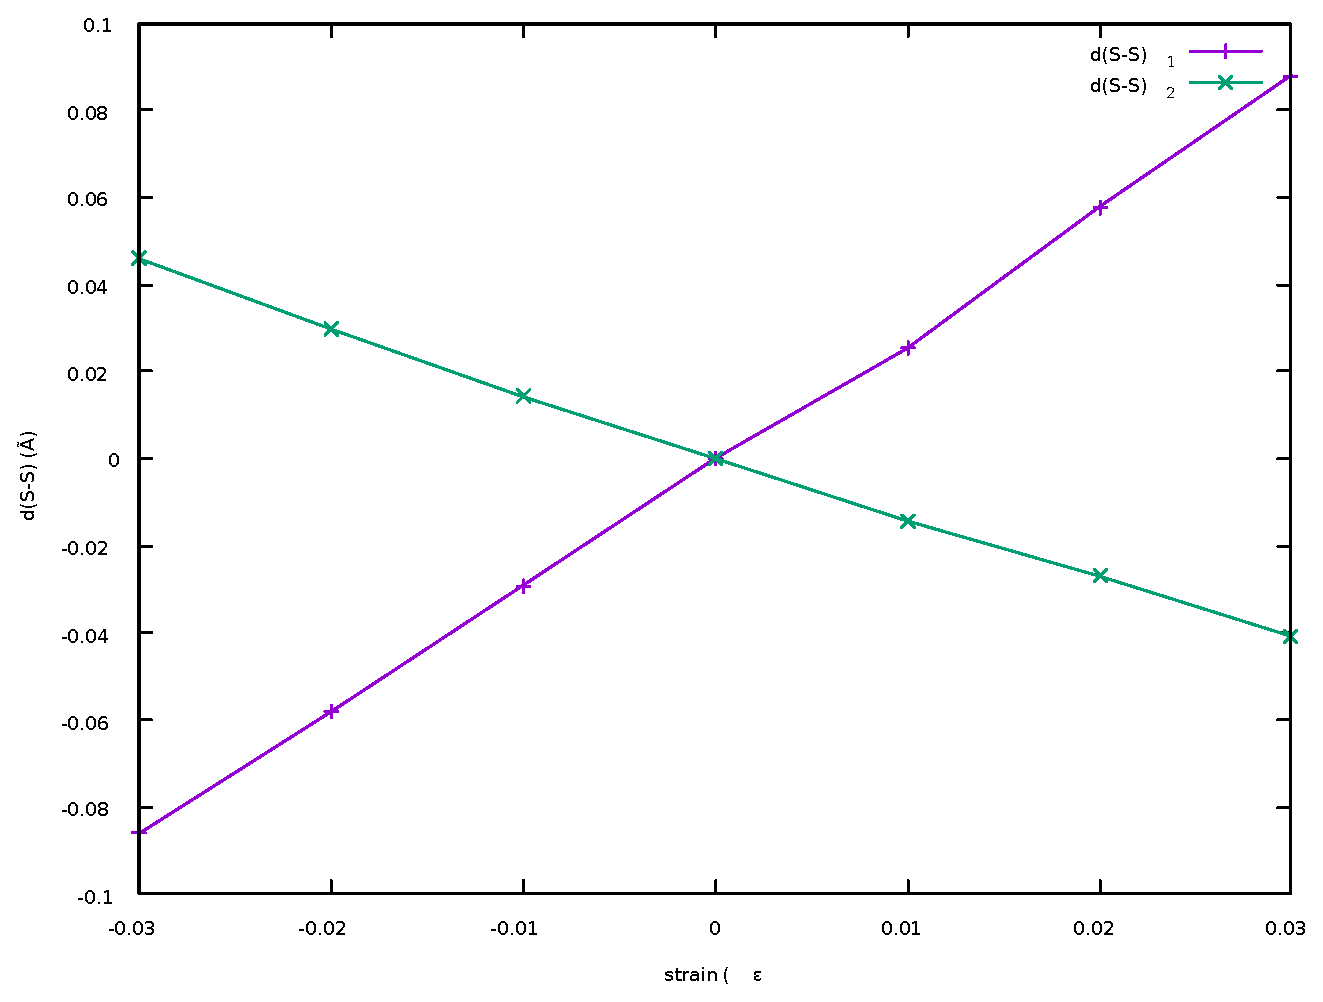
\epsfig{file=figRes/PtS2/anis/compS.eps, width=7.0cm,height=7.0cm}
		%\caption{Strain isotr\'opico}
		\label{fig:compdSpt}
	\end{figure}
}

\frame{\frametitle{$PtS_2$}
	\framesubtitle{comparativo $\Delta Pt-S $}
	
	\begin{figure}[!hbt]
		\centering
		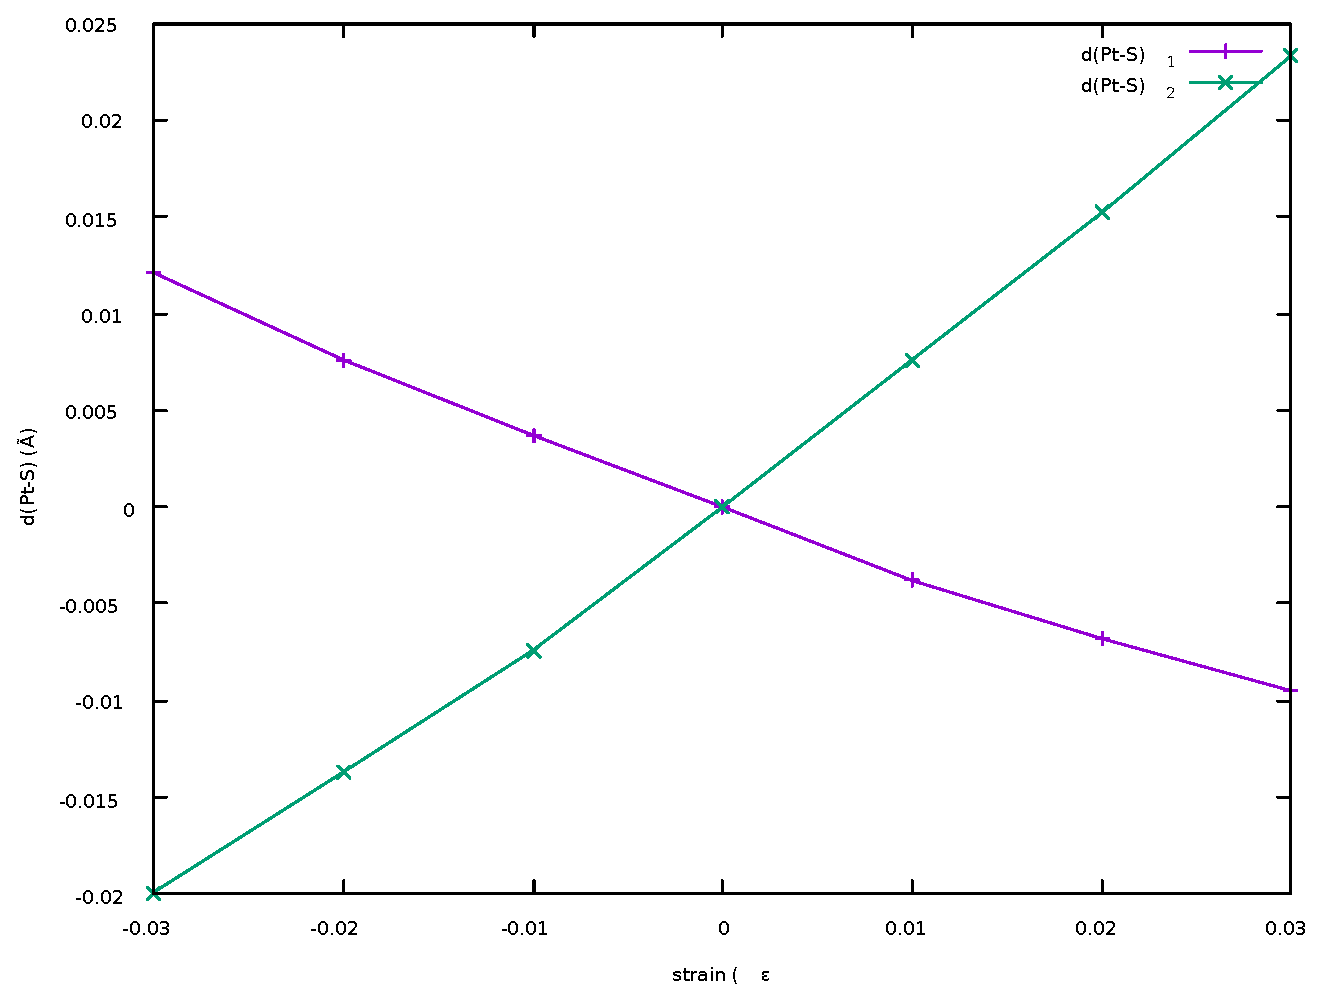
\epsfig{file=figRes/PtS2/anis/compPtS.eps, width=7.0cm,height=7.0cm}
		%\caption{Strain isotr\'opico}
		\label{fig:compdSePt1}
	\end{figure}
}
\frame{\frametitle{$PtS_2$}
	\framesubtitle{$\Delta Pt $}
	
	\begin{figure}[!hbt]
		\centering
		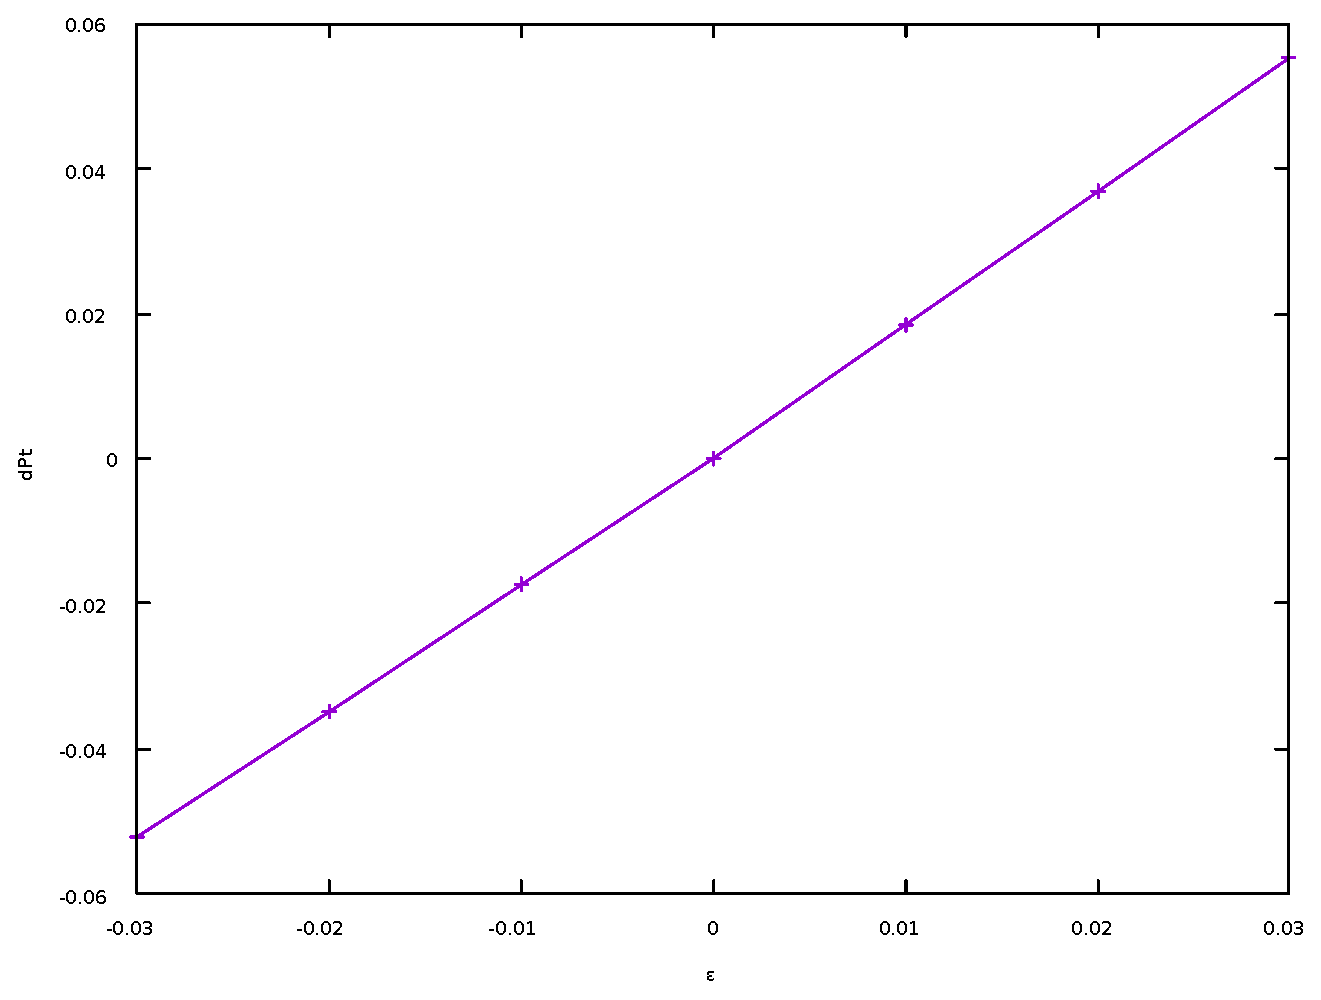
\epsfig{file=figRes/PtS2/anis/dPt.eps, width=7.0cm,height=7.0cm}
		%\caption{Strain isotr\'opico}
		\label{fig:dPt2}
	\end{figure}
}

\frame{\frametitle{$PtSe_2$}
	\framesubtitle{ comparativo $\Delta Se $}
	
	\begin{figure}[!hbt]
		\centering
		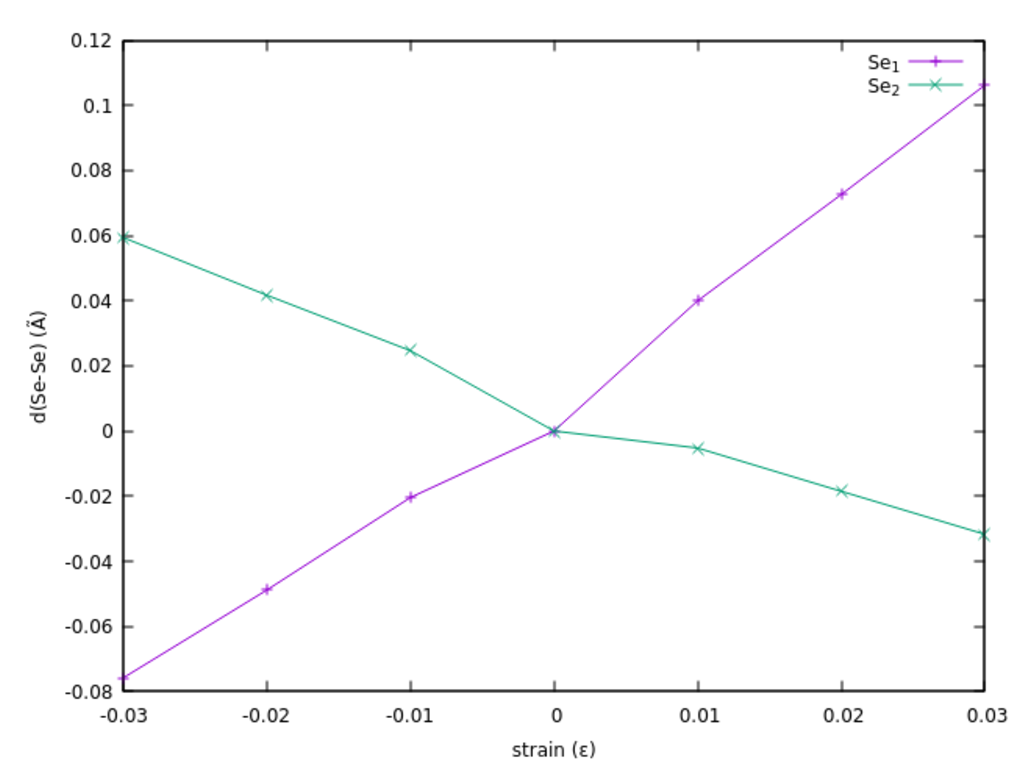
\epsfig{file=figRes/PtSe2/ans/compS.eps, width=7.0cm,height=7.0cm}
		%\caption{Strain isotr\'opico}
		\label{fig:comsdSe3}
	\end{figure}
}

\frame{\frametitle{$PtSe_2$}
	\framesubtitle{comparativo $\Delta Pt-Se $}
	
	\begin{figure}[!hbt]
		\centering
		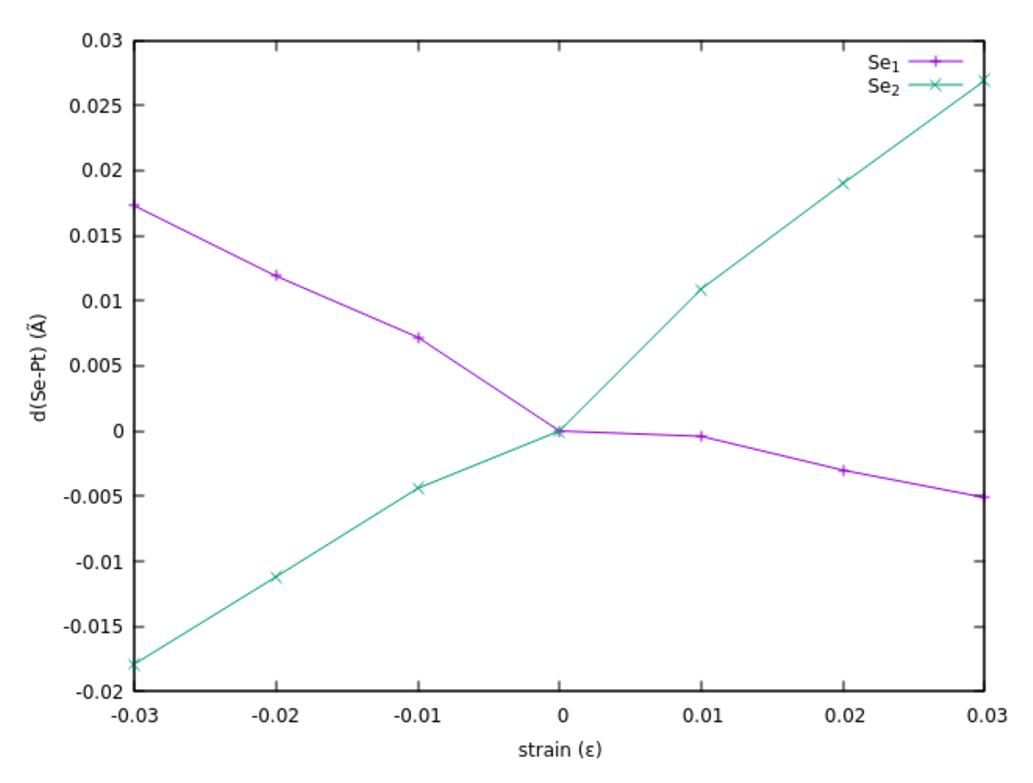
\epsfig{file=figRes/PtSe2/ans/compSPt.eps, width=7.0cm,height=7.0cm}
		%\caption{Strain isotr\'opico}
		\label{fig:compdSPt}
	\end{figure}
}
\frame{\frametitle{$PtSe_2$}
	\framesubtitle{$\Delta Pt $}
	
	\begin{figure}[!hbt]
		\centering
		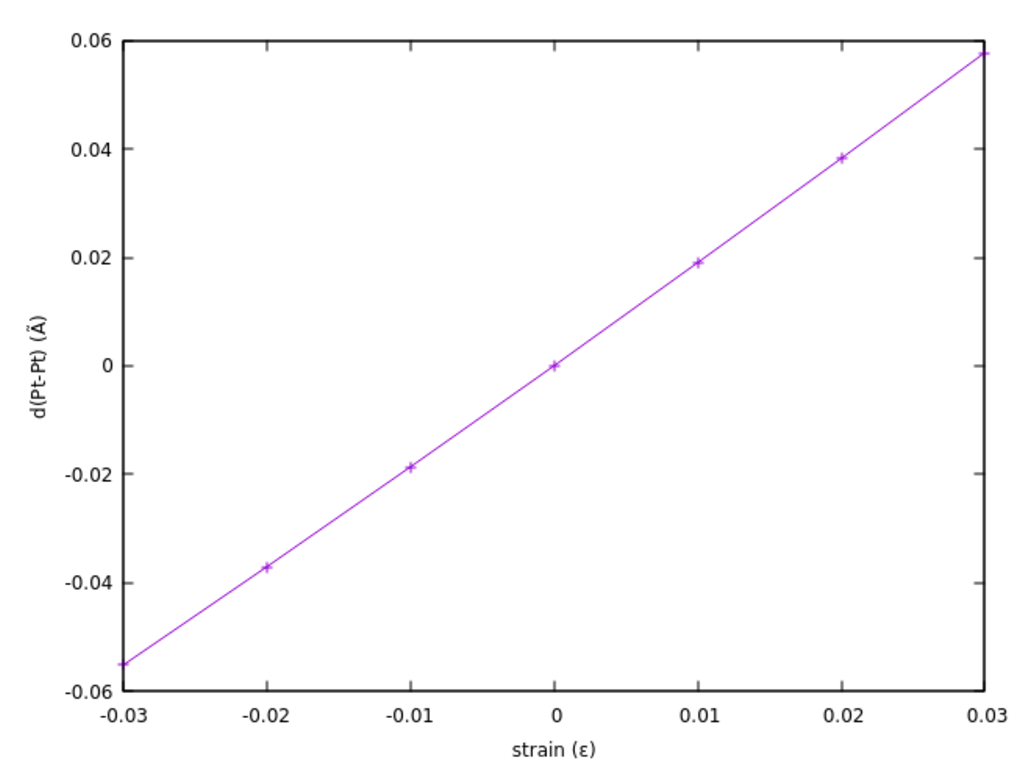
\epsfig{file=figRes/PtSe2/ans/dPt.eps, width=7.0cm,height=7.0cm}
		%\caption{Strain isotr\'opico}
		\label{fig:dPt3}
	\end{figure}
}
\subsection{vacancia de metal de transici\'on }

\frame{\frametitle{strain isotr\'opico}
	%$\varepsilon = \frac{a-a_1}{a_1} $
	\begin{figure}[!hbt]
		\centering
		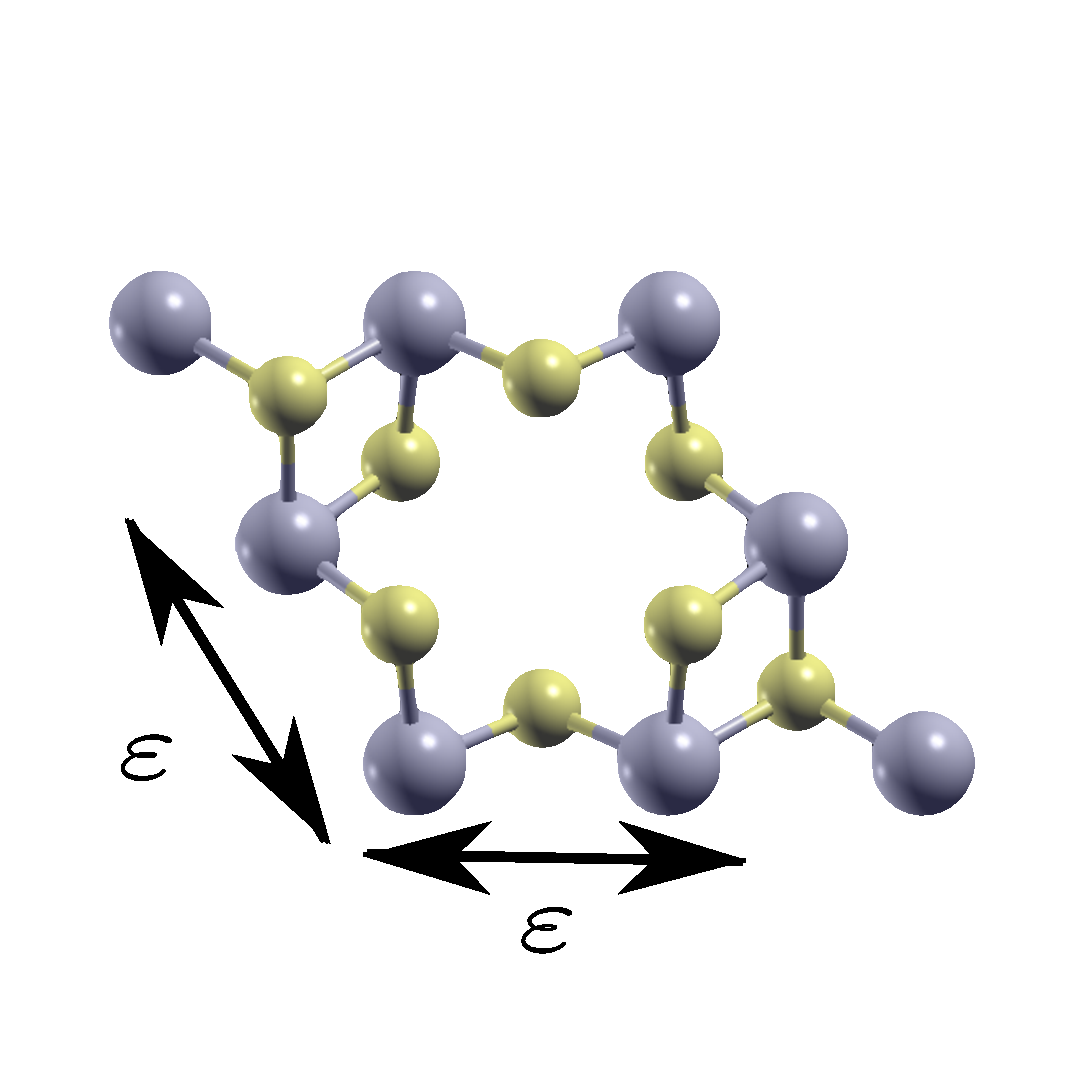
\epsfig{file=figRes/strainIsoDef.eps, width=7.0cm,height=7.0cm}
		%\caption{Strain isotr\'opico}
		\label{fig:strIsoU}
	\end{figure}
}
\frame{\frametitle{distancias}
	\begin{figure}[!hbt]
		\centering
		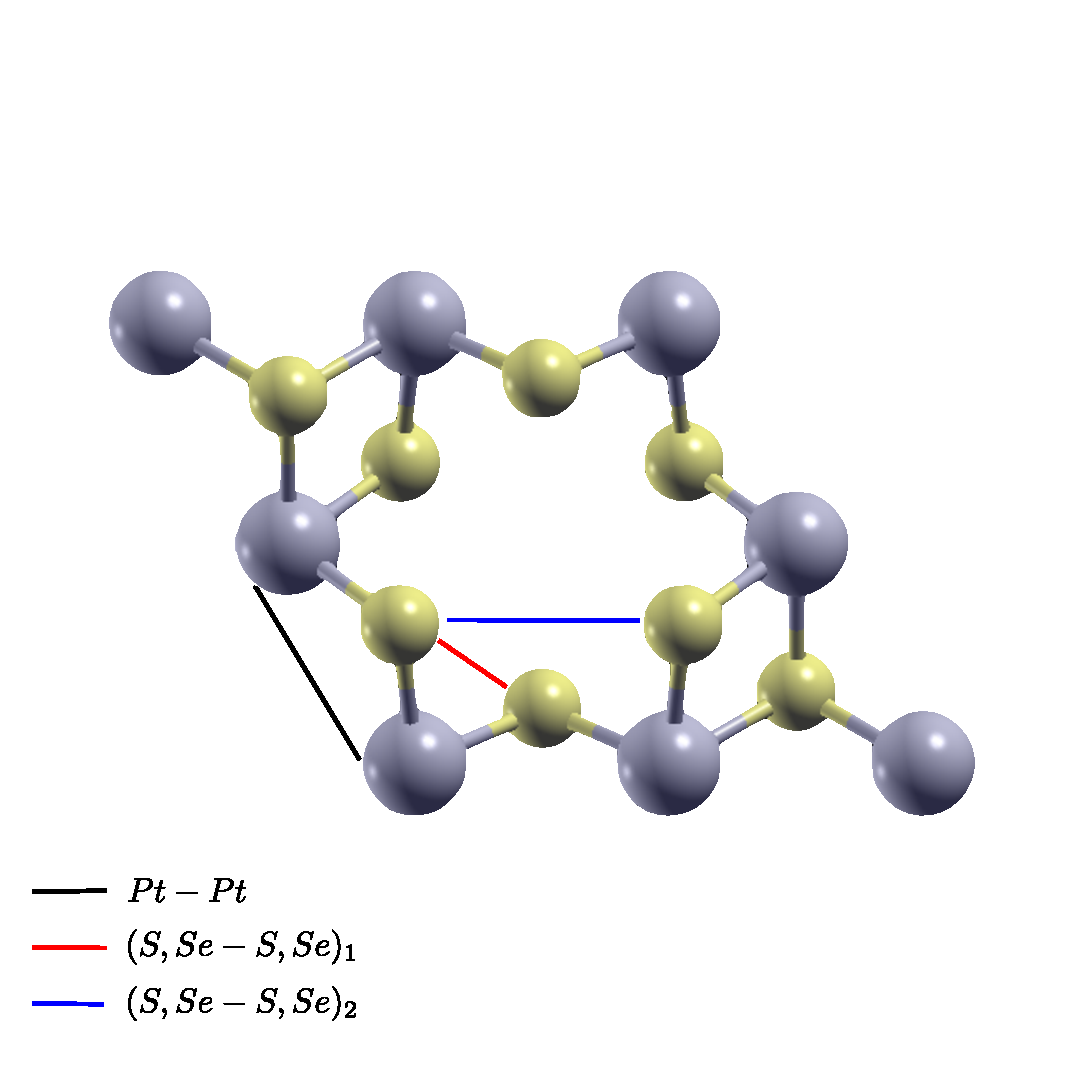
\epsfig{file=figRes/compIsoDef.eps, width=7.0cm,height=7.0cm}
		%\caption{Strain isotr\'opico}
		\label{fig:strIsoUComp}
	\end{figure}
}

\frame{
	\frametitle{$PtS_2$}
	\framesubtitle{magnetizaci\'on}
	
	\begin{figure}[!hbt]
		\centering
		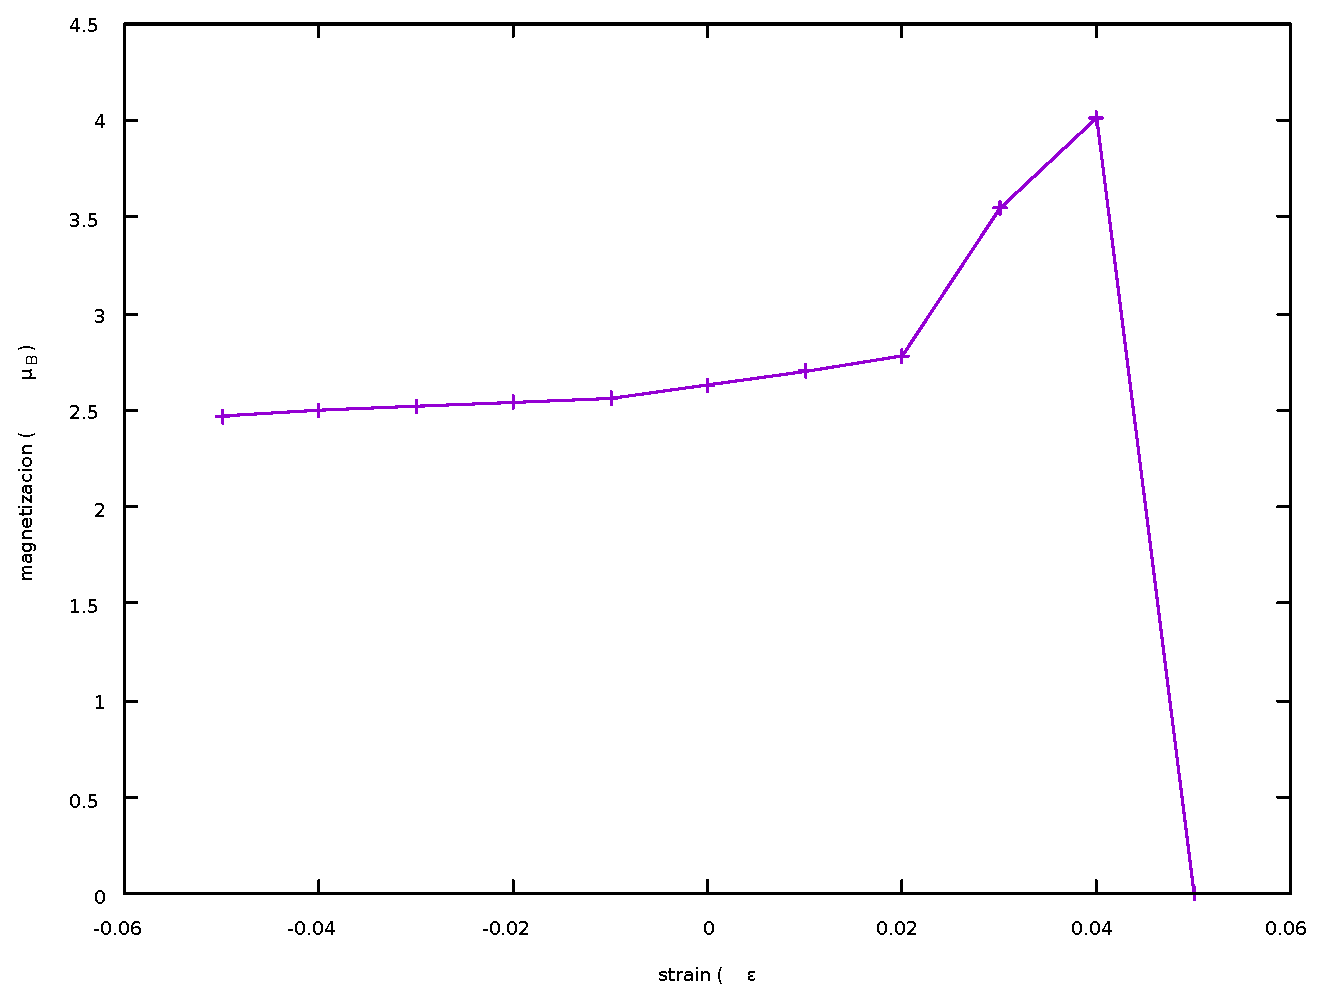
\epsfig{file=figRes/PtS2/def/iso/magn.eps, width=7.0cm,height=7.0cm}
		%\caption{Strain isotr\'opico}
		\label{fig:PtSe21}
	\end{figure}
}

\frame{\frametitle{$PtS_2$}
	\framesubtitle{comparativo $\Delta S $}
	
	\begin{figure}[!hbt]
		\centering
		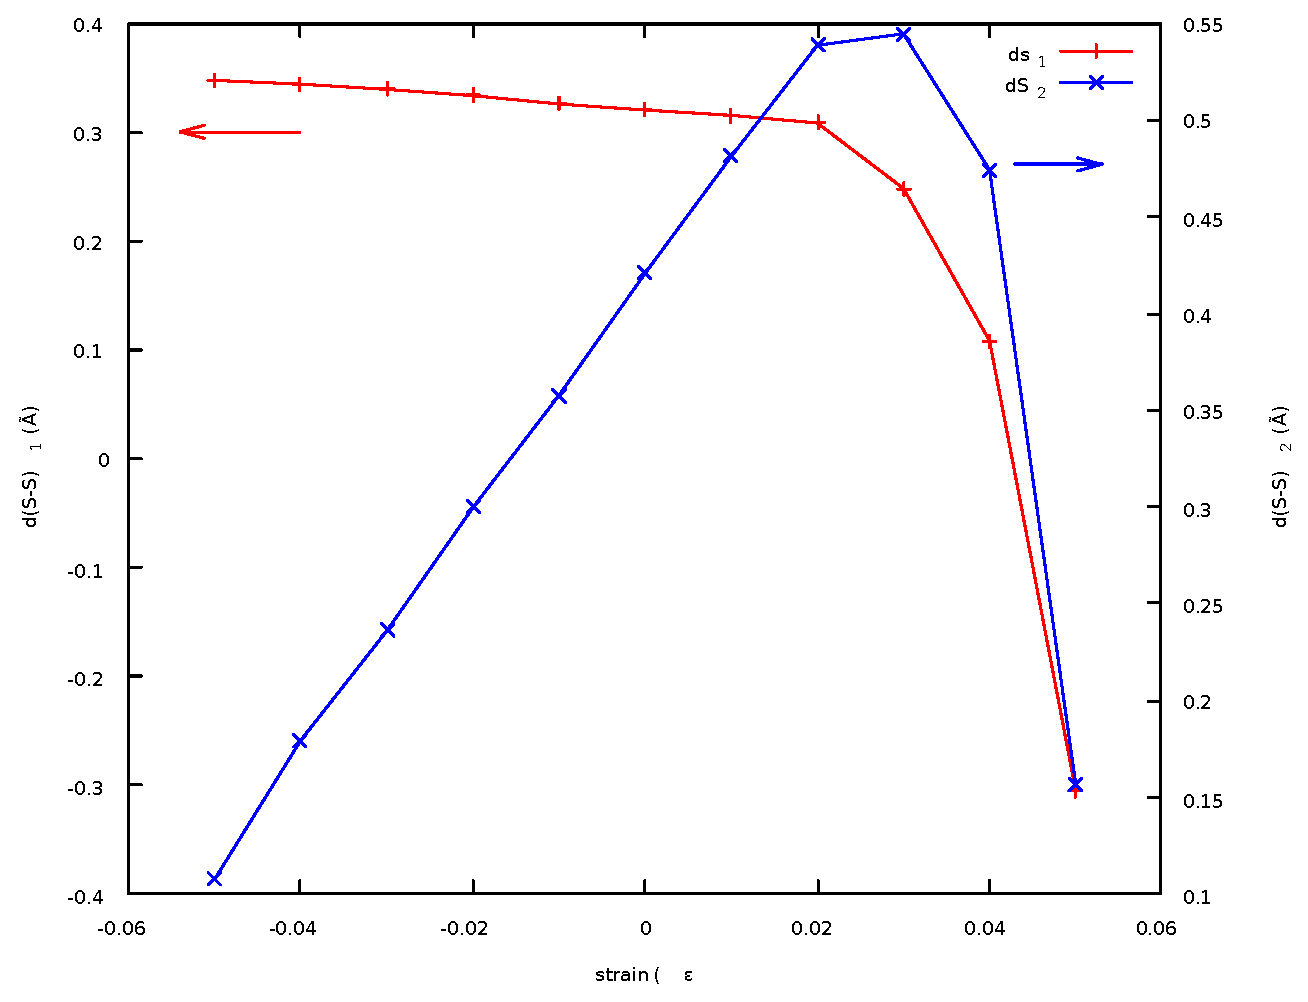
\epsfig{file=figRes/PtS2/def/iso/compS.eps, width=7.0cm,height=7.0cm}
		%\caption{Strain isotr\'opico}
		\label{fig:dS3}
	\end{figure}
}


\frame{\frametitle{$PtS_2$}
	\framesubtitle{$\Delta Pt $}
	
	\begin{figure}[!hbt]
		\centering
		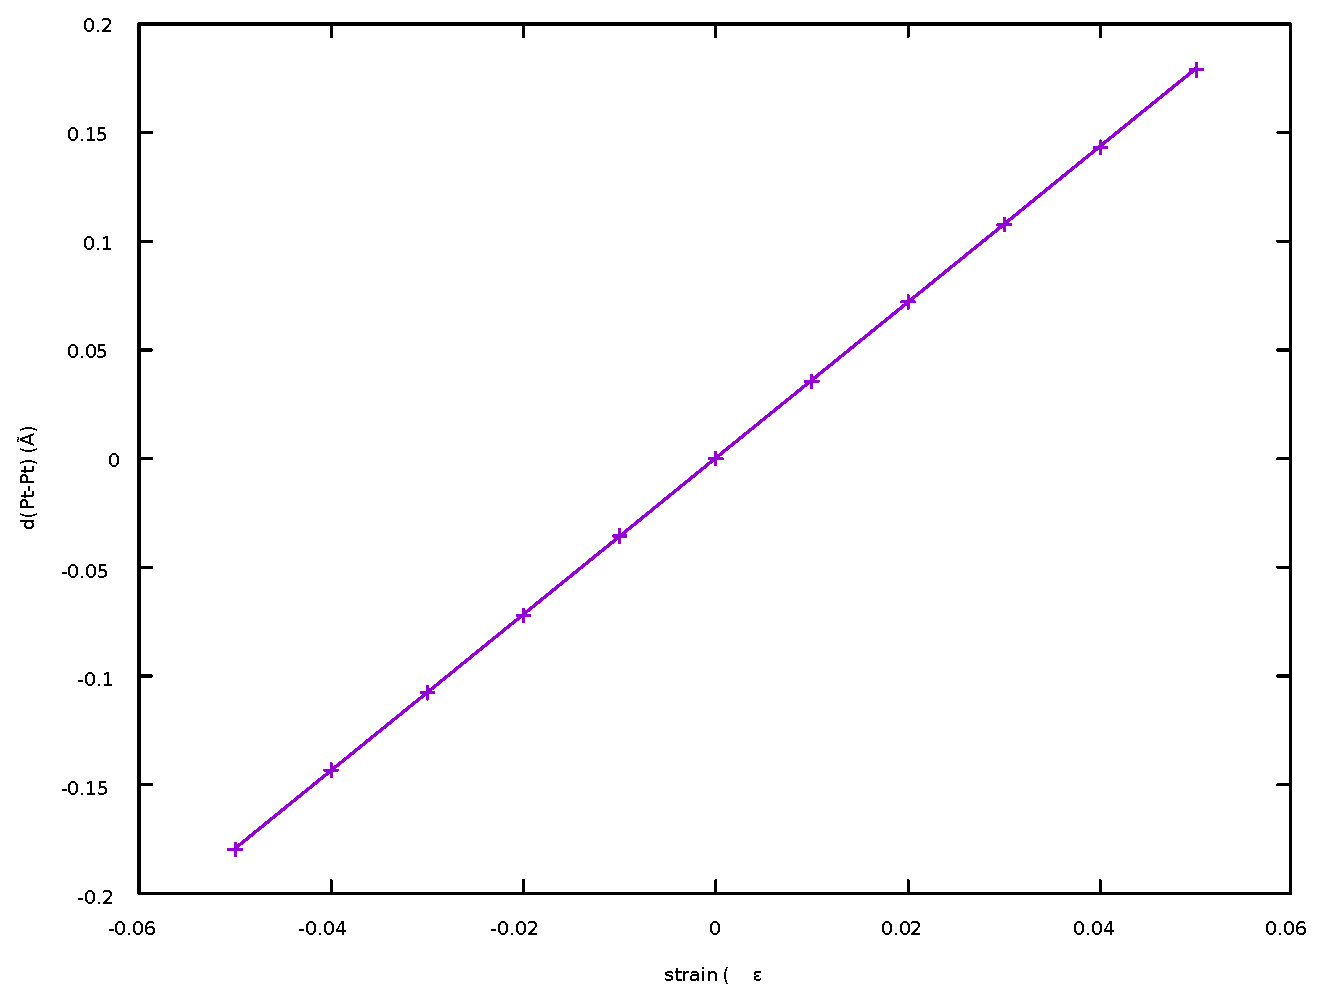
\epsfig{file=figRes/PtS2/def/iso/dPt.eps, width=7.0cm,height=7.0cm}
		%\caption{Strain isotr\'opico}
		\label{fig:dPt1}
	\end{figure}
}

\frame{\frametitle{$PtSe_2$}
	\framesubtitle{magnetizaci\'on}
	
	\begin{figure}[!hbt]
		\centering
		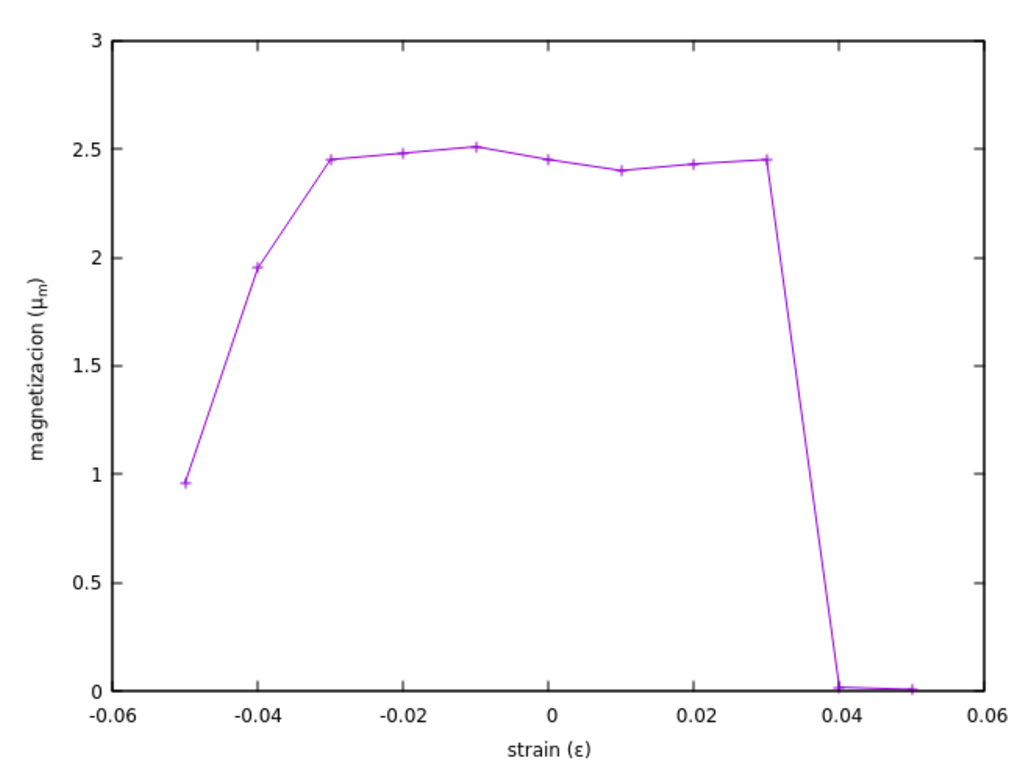
\epsfig{file=figRes/PtSe2/def/iso/magn.eps, width=7.0cm,height=7.0cm}
		%\caption{Strain isotr\'opico}
		\label{fig:dSPt1}
	\end{figure}
}

\frame{\frametitle{$PtSe_2$}
	\framesubtitle{comparativo $\Delta Se $}
	
	\begin{figure}[!hbt]
		\centering
		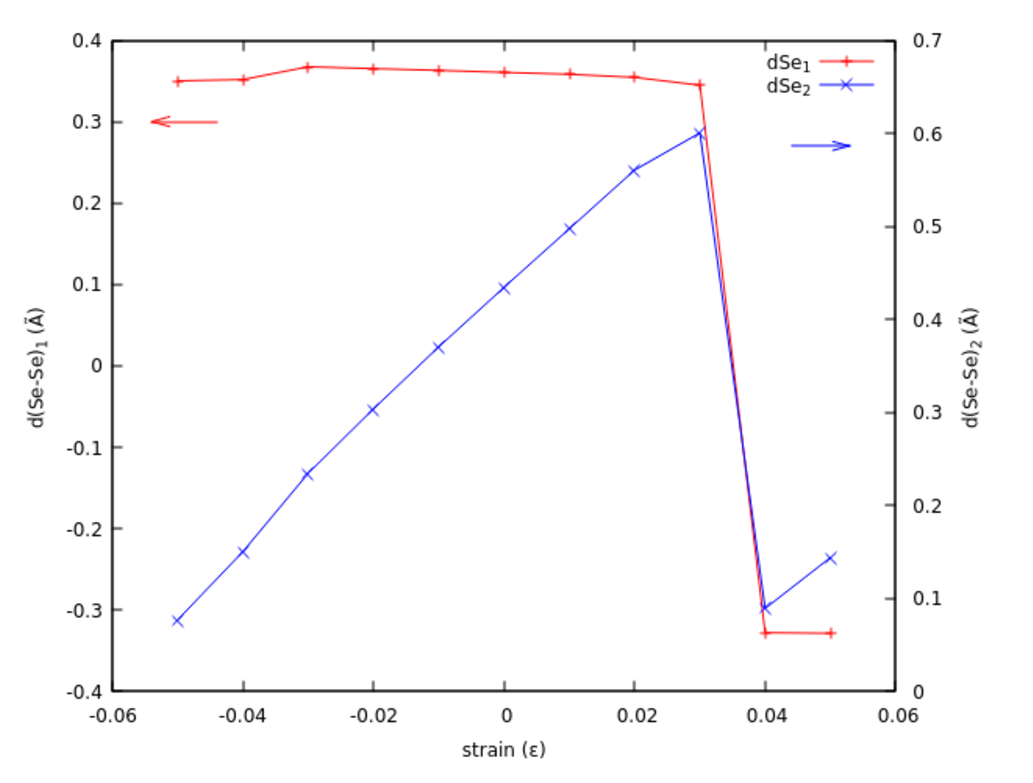
\epsfig{file=figRes/PtSe2/def/iso/compSe.eps, width=7.0cm,height=7.0cm}
		%\caption{Strain isotr\'opico}
		\label{fig:dSe3}
	\end{figure}
}


\frame{\frametitle{$PtSe_2$}
	\framesubtitle{$\Delta Pt $}
	
	\begin{figure}[!hbt]
		\centering
		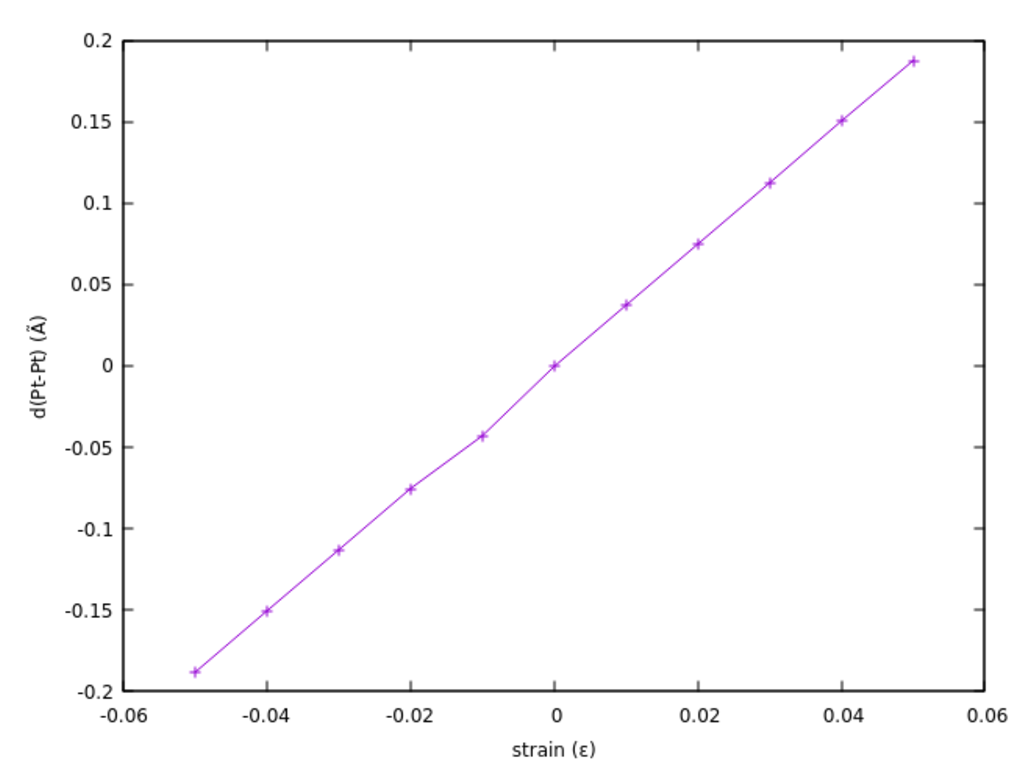
\epsfig{file=figRes/PtSe2/def/iso/dPt.eps, width=7.0cm,height=7.0cm}
		%\caption{Strain isotr\'opico}
		\label{fig:dPt2}
	\end{figure}
}

\frame{\frametitle{strain anisotr\'opico}
	$\varepsilon = \frac{a-a_1}{a_1} $
	\begin{figure}[!hbt]
		\centering
		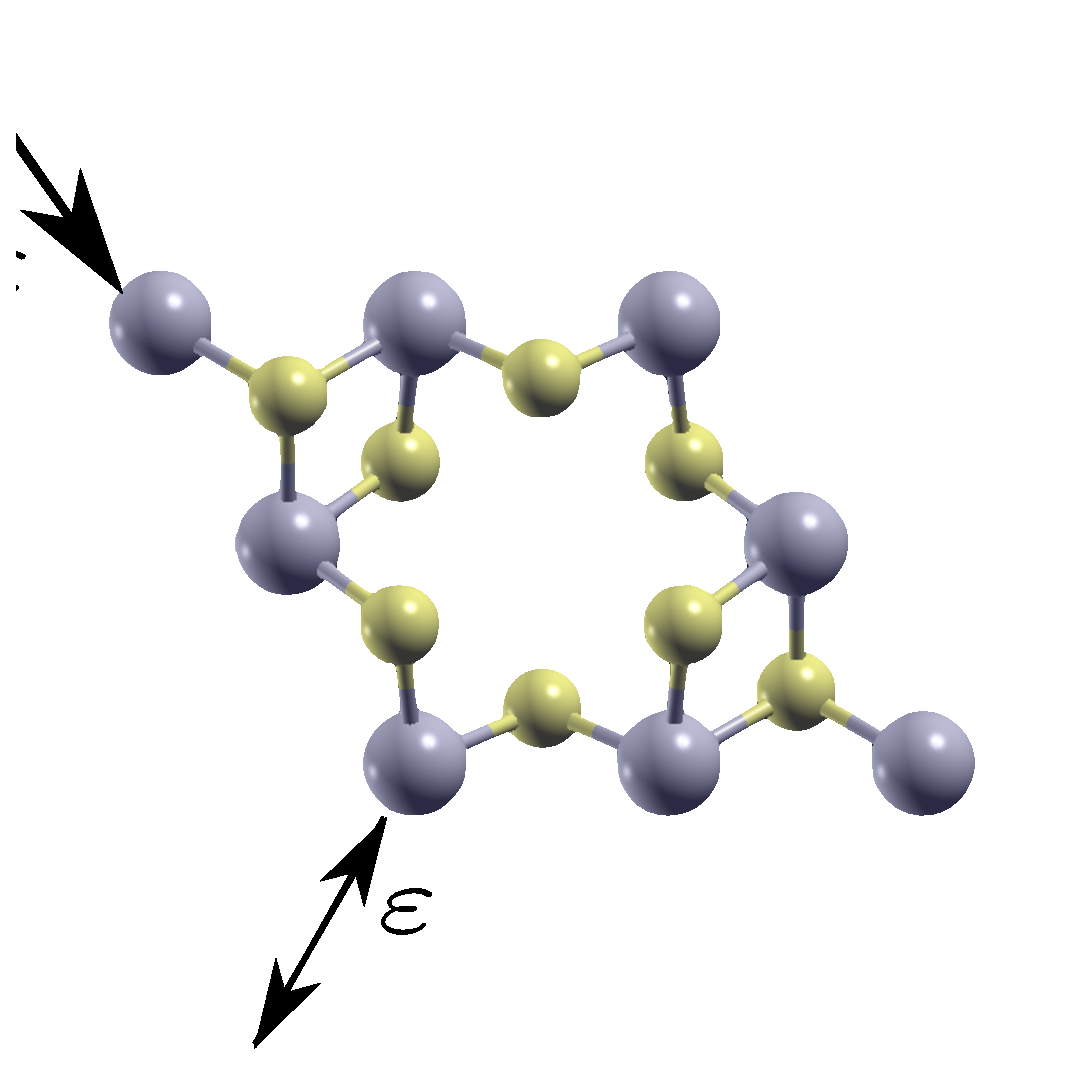
\epsfig{file=figRes/strainAnisDef.eps, width=5.0cm,height=5.0cm}
		%\caption{Strain isotr\'opico}
		\label{fig:strAnisU}
	\end{figure}
}
\frame{\frametitle{distancias}
	\begin{figure}[!hbt]
		\centering
		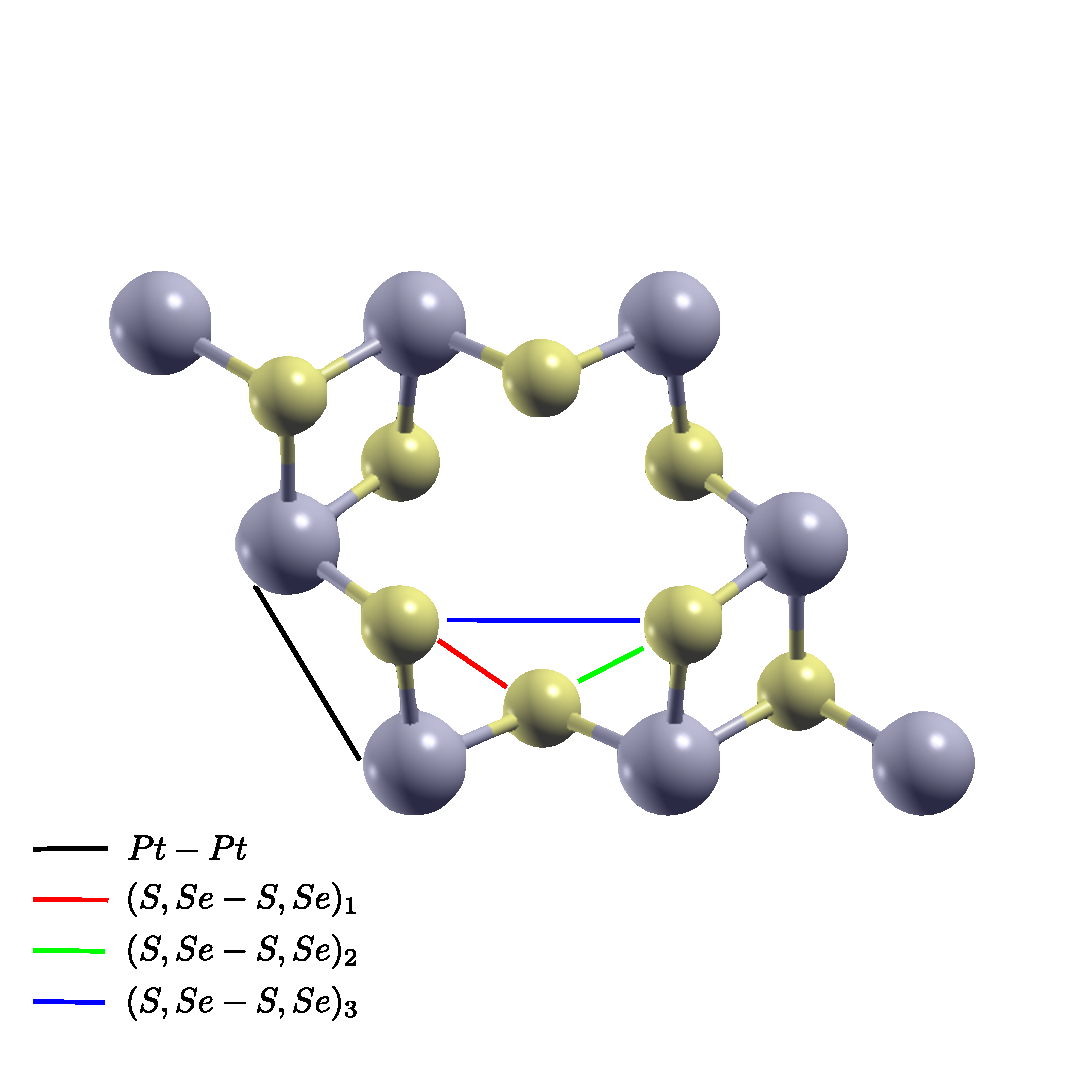
\epsfig{file=figRes/compAnisDef.eps, width=7.0cm,height=7.0cm}
		%\caption{Strain isotr\'opico}
		\label{fig:strAnisUComp}
	\end{figure}
}

\frame{
	\frametitle{$PtS_2$}
	\framesubtitle{magnetizaci\'on}
	
	\begin{figure}[!hbt]
		\centering
		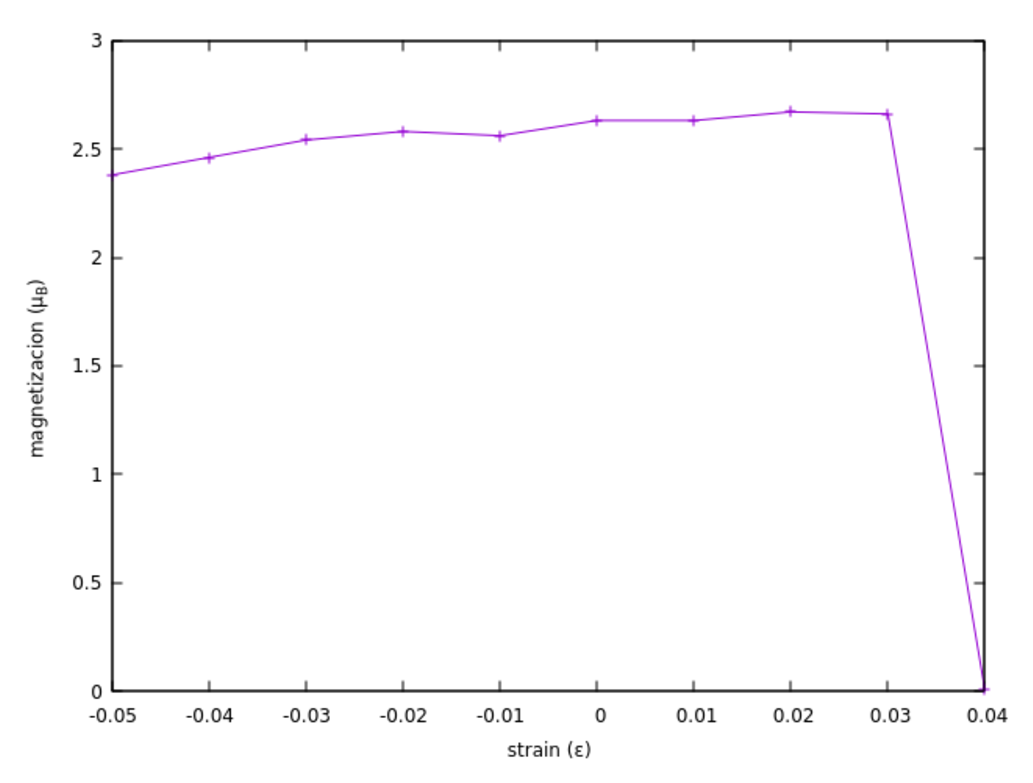
\epsfig{file=figRes/PtS2/def/anis/magn.eps, width=7.0cm,height=7.0cm}
		%\caption{Strain isotr\'opico}
		\label{fig:PtSe21}
	\end{figure}
}

\frame{\frametitle{$PtS_2$}
	\framesubtitle{comparativo $\Delta S_{1,2} $}
	
	\begin{figure}[!hbt]
		\centering
		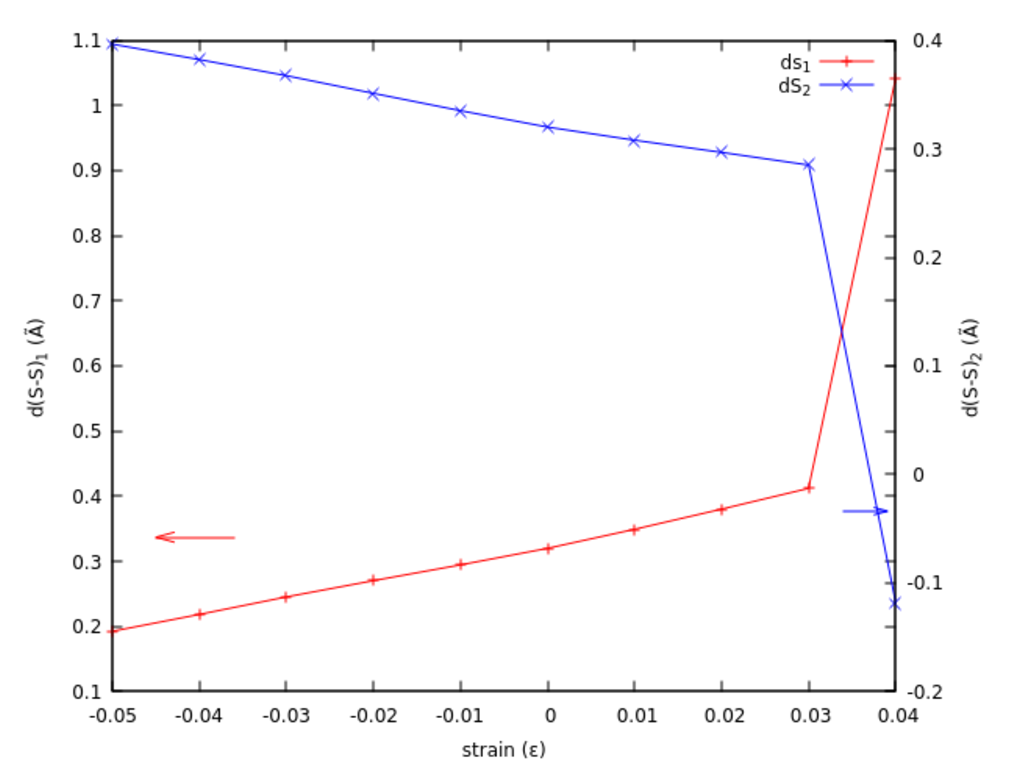
\epsfig{file=figRes/PtS2/def/anis/compdS12.eps, width=7.0cm,height=7.0cm}
		%\caption{Strain isotr\'opico}
		\label{fig:dS3}
	\end{figure}
}

\frame{\frametitle{$PtS_2$}
	\framesubtitle{comparativo $\Delta S_{2,3} $}
	
	\begin{figure}[!hbt]
		\centering
		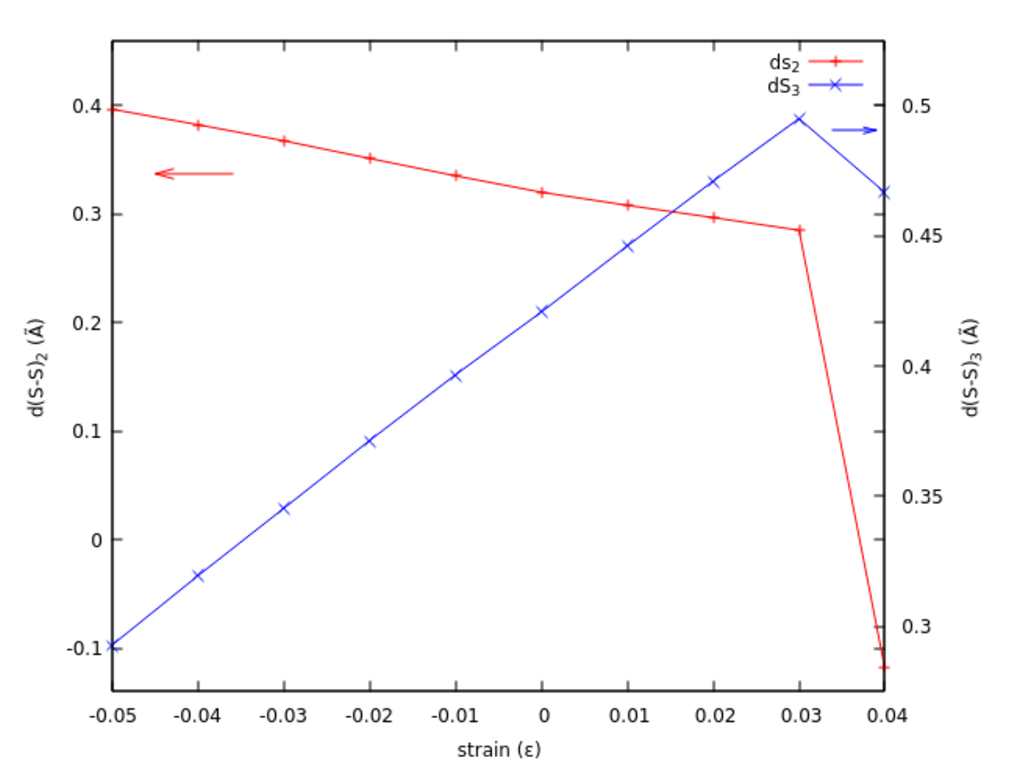
\epsfig{file=figRes/PtS2/def/anis/compdS23.eps, width=7.0cm,height=7.0cm}
		%\caption{Strain isotr\'opico}
		\label{fig:dS3}
	\end{figure}
}

\frame{\frametitle{$PtS_2$}
	\framesubtitle{$\Delta Pt $}
	
	\begin{figure}[!hbt]
		\centering
		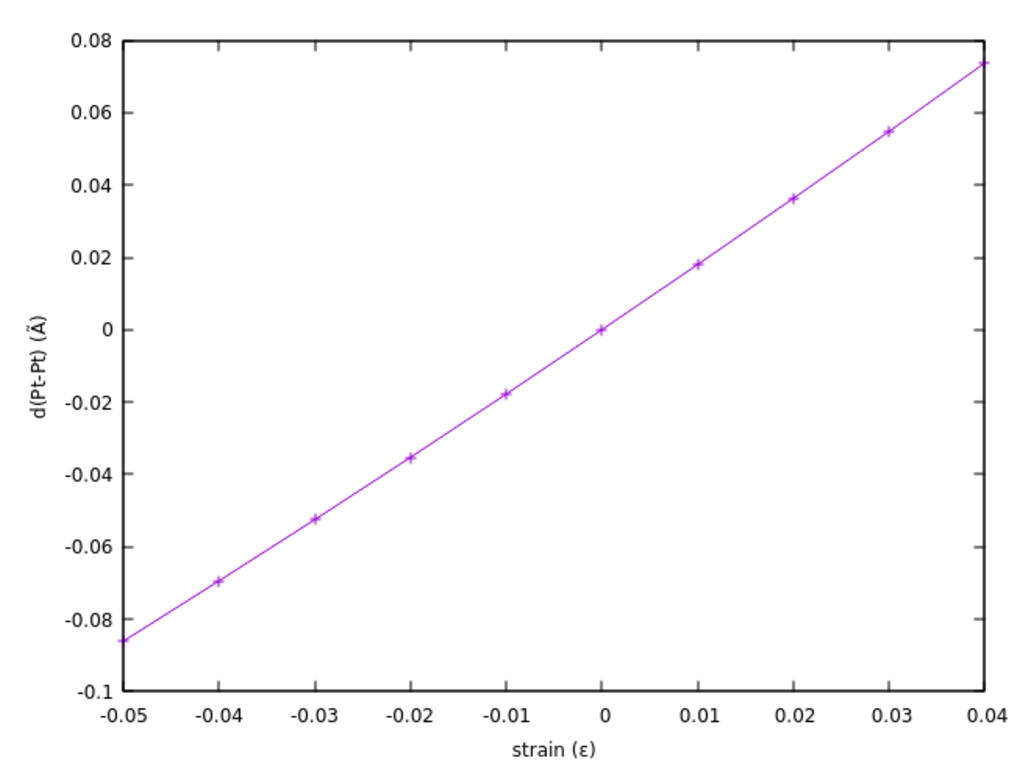
\epsfig{file=figRes/PtS2/def/anis/dPt.eps, width=7.0cm,height=7.0cm}
		%\caption{Strain isotr\'opico}
		\label{fig:dPt1}
	\end{figure}
}
\frame{\frametitle{deformaci\'on de $\varepsilon=0.04$}
    \begin{figure}[!hbt]
    	\centering
    	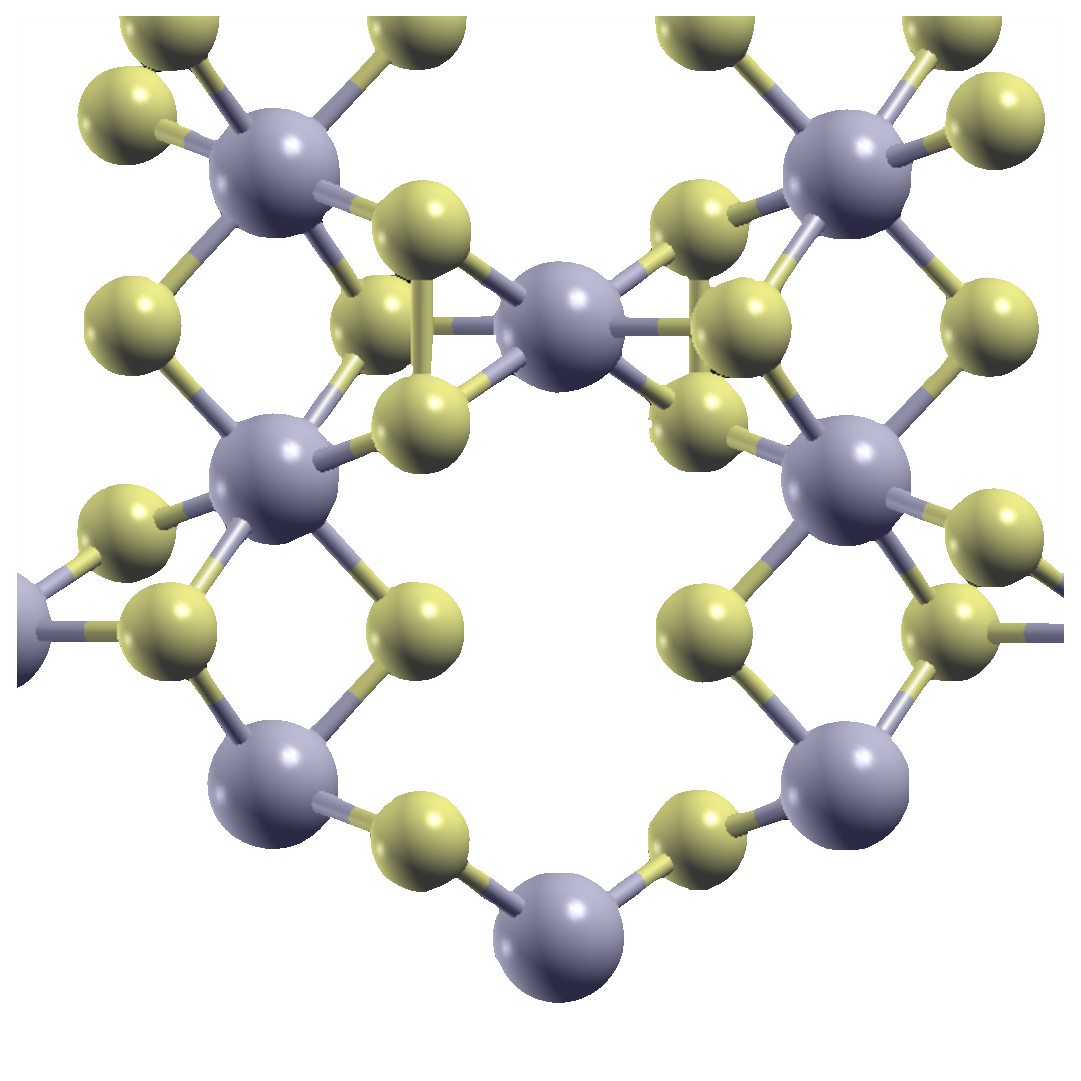
\epsfig{file=figRes/PtS2_0.04_Anis.eps, width=7.0cm,height=7.0cm}
    	%\caption{Strain isotr\'opico}
    	\label{fig:strAnisUComp}
    \end{figure}
}


\frame{\frametitle{$PtSe_2$}
	\framesubtitle{magnetizaci\'on}
	
	\begin{figure}[!hbt]
		\centering
		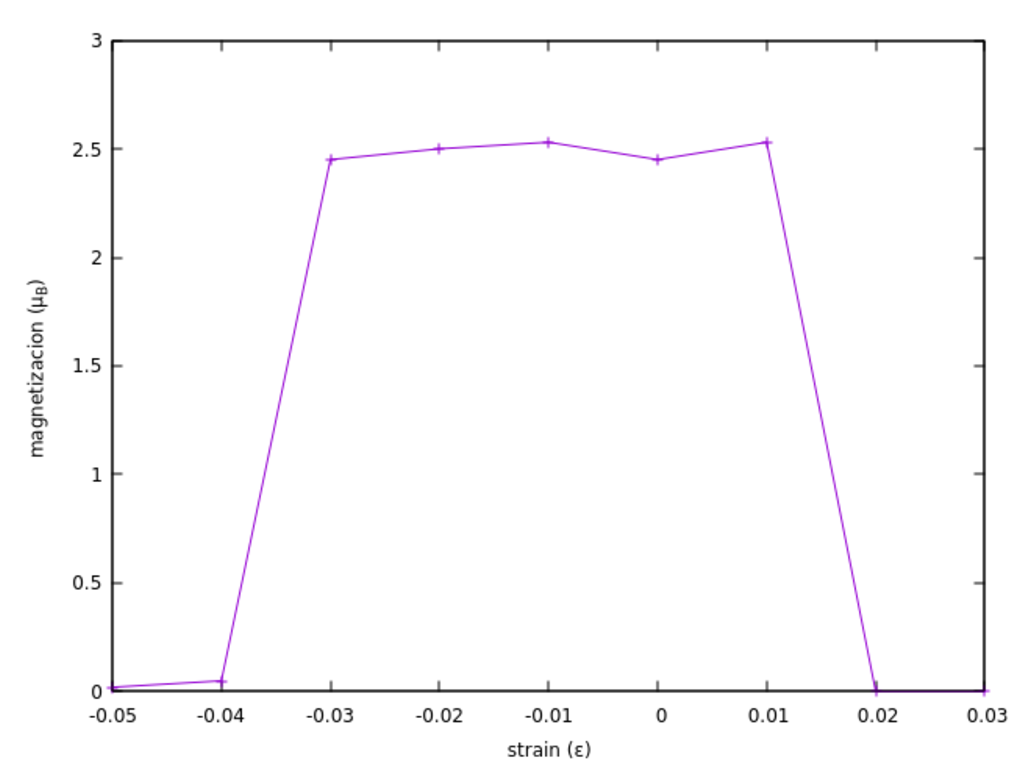
\epsfig{file=figRes/PtSe2/def/anis/magn.eps, width=7.0cm,height=7.0cm}
		%\caption{Strain isotr\'opico}
		\label{fig:dSPt1}
	\end{figure}
}

\frame{\frametitle{$PtSe_2$}
	\framesubtitle{comparativo $\Delta Se $}
	
	\begin{figure}[!hbt]
		\centering
		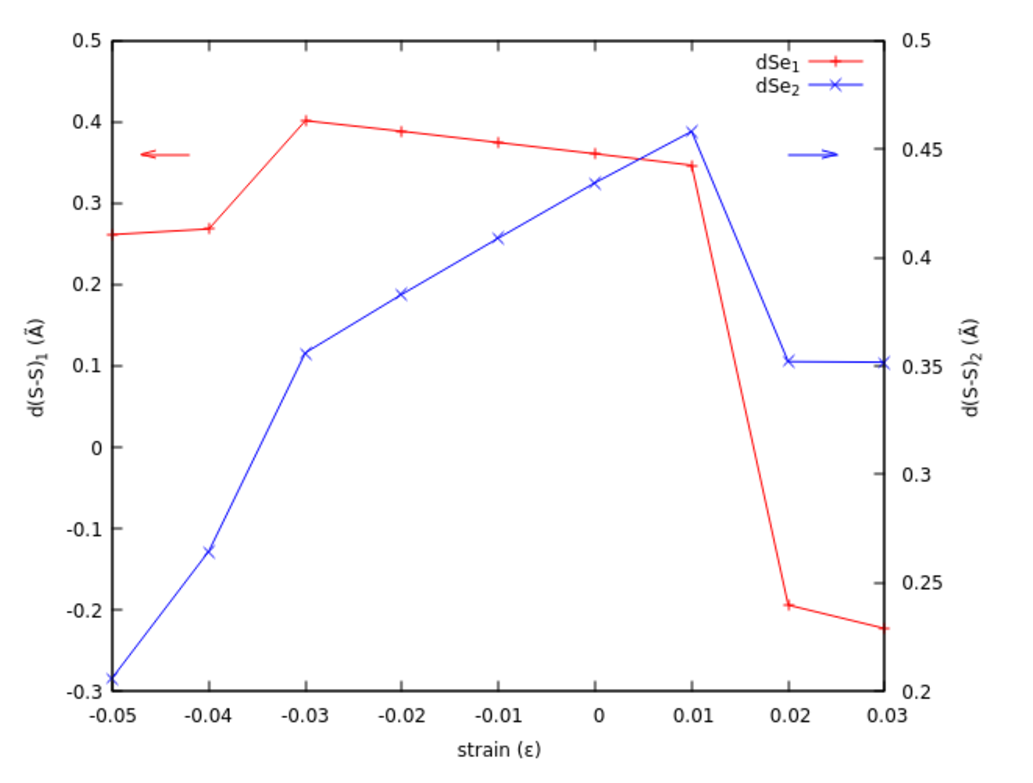
\epsfig{file=figRes/PtSe2/def/anis/compSe.eps, width=7.0cm,height=7.0cm}
		%\caption{Strain isotr\'opico}
		\label{fig:dSe3}
	\end{figure}
}

\frame{\frametitle{$PtSe_2$}
	\framesubtitle{ $\Delta Se_3 $}
	
	\begin{figure}[!hbt]
		\centering
		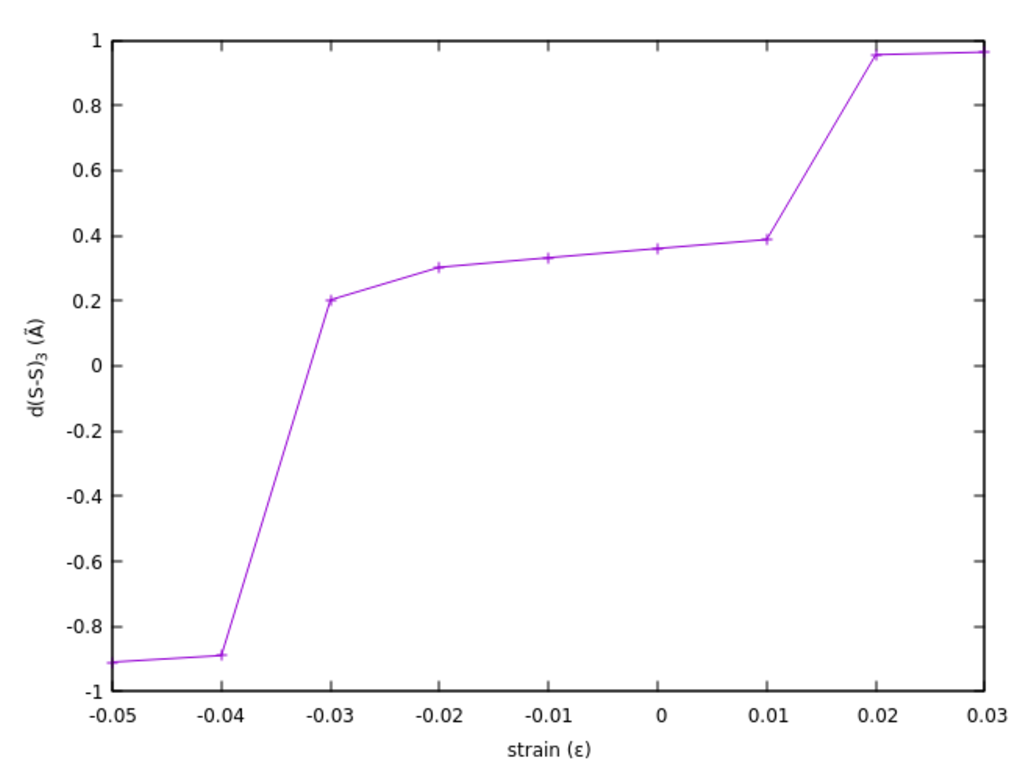
\epsfig{file=figRes/PtSe2/def/anis/dS3.eps, width=7.0cm,height=7.0cm}
		%\caption{Strain isotr\'opico}
		\label{fig:dSe3}
	\end{figure}
}

\frame{\frametitle{$PtSe_2$}
	\framesubtitle{$\Delta Pt $}
	
	\begin{figure}[!hbt]
		\centering
		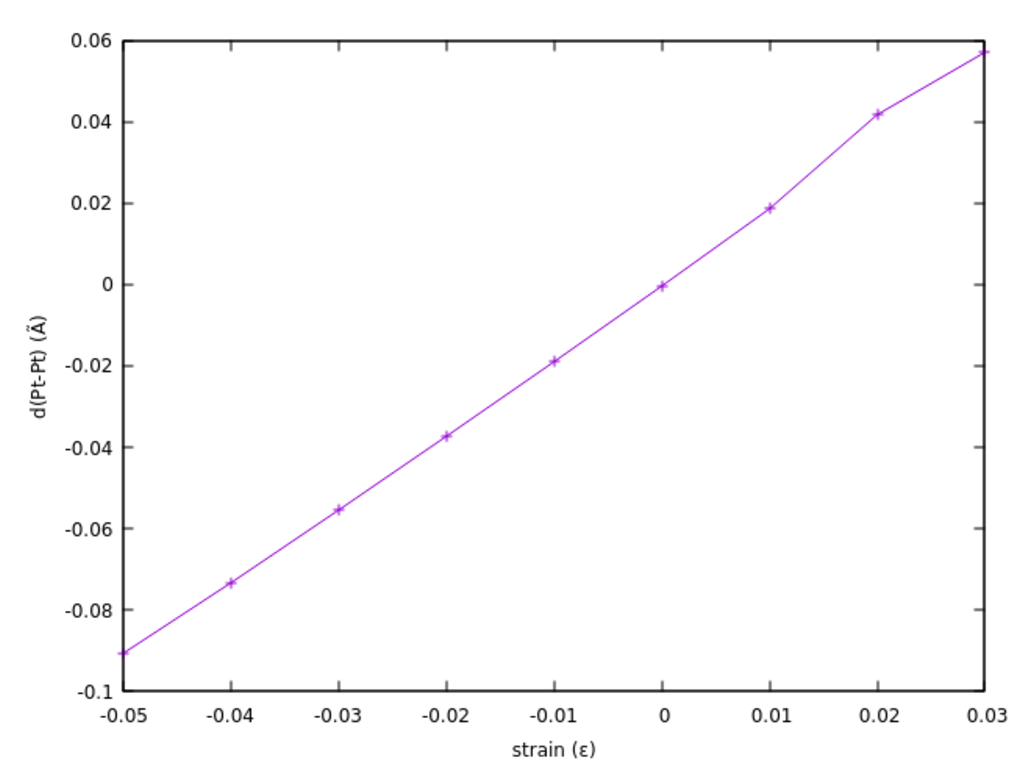
\epsfig{file=figRes/PtSe2/def/anis/dPt.eps, width=7.0cm,height=7.0cm}
		%\caption{Strain isotr\'opico}
		\label{fig:dPt2}
	\end{figure}
}
\frame{\frametitle{deformaci\'on de $\varepsilon=-0.05$}
	\begin{figure}[!hbt]
		\centering
		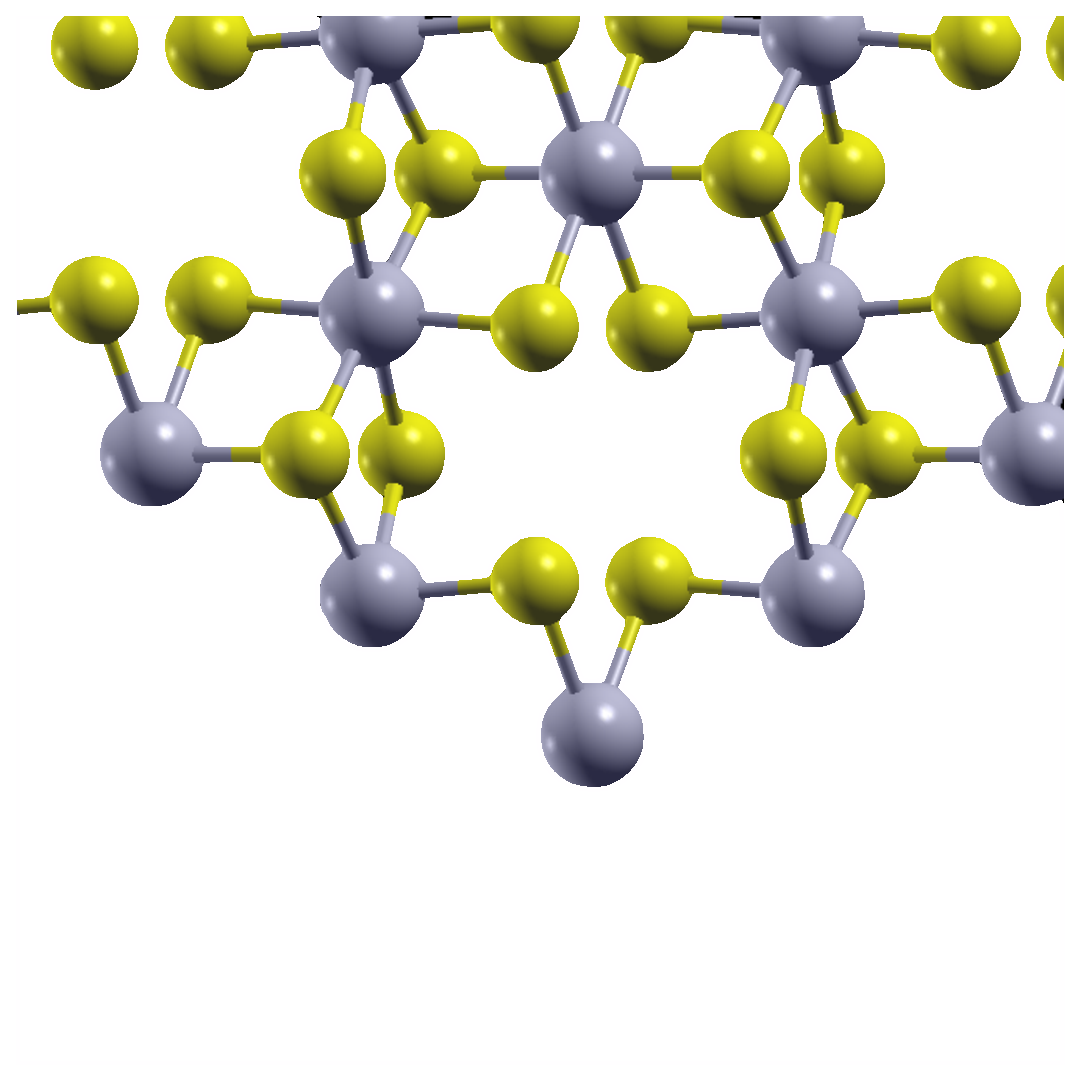
\epsfig{file=figRes/PtSe2_-0.05_anis.eps, width=7.0cm,height=7.0cm}
		%\caption{Strain isotr\'opico}
		\label{fig:strAnisUComp}
	\end{figure}
}
\frame{\frametitle{deformaci\'on de $\varepsilon=0.03$}
	\begin{figure}[!hbt]
		\centering
		\epsfig{file=figRes/PtSe2_0.03_anis.eps, width=7.0cm,height=7.0cm}
		%\caption{Strain isotr\'opico}
		\label{fig:strAnisUComp}
	\end{figure}
}
\end{document}